\FloatBarrier
\subsection{Main interferometer optical components}\label{sec:optcomps}
%\emph{Author(s): \textbf{K.\ Kokeyama}, A.\ Freise, etc.}\\

The materials for the optical components for the ET HF and LF detector have to be chosen taking different factors into account: the optical properties, mechanical properties as well as thermal properties. The ET HF interferometer will be based on the first and second generation of GW detectors and will use fused silica for all optical components. This material is currently state of the art in precision optics. The ET HF detector will be operated at room temperature.

The ET LF interferometer has to be built from crystalline materials due to thermal noise requirements which will be described in this section. Possible materials that fulfill the mentioned demands are silicon and sapphire. These materials will be operated at cryogenic temperatures. The following sections contain detailed discussions of the material properties, their mechanical and thermal properties and the detailed description of the thermal noise arising from the different materials. The material properties are summarised in Appendix\,\ref{sec:app}. The final outcome of this section will be the definition of the geometry of the test masses - as summarised in Appendix \ref{sec:layoutparams} - due to thermal noise requirements. Additionally, we describe the optimum operational temperature of ET LF which was found to be 10\,K.

\FloatBarrier
\subsubsection{Bulk material selection}
\label{sec:material}

%\emph{Authors: J. Franc, K. Kokeyama, R. Nawrodt}

Different materials have been proposed in order to reduce the thermal noise of the optics of future gravitational wave detectors. Three main candidate materials are the most promising ones to construct a 3rd generation detector: fused silica, sapphire and silicon.

{\bf Fused silica} is the favorite substrate material for an interferometer that operates at room temperature. It is the substrate material of advanced detectors like Advanced LIGO and Advanced Virgo. Due to the extensive use of fused silica for first and second generation gravitational wave detectors, this material has been extensively characterised at room temperature. Fused silica exhibits very low optical absorption (as low as 1\,ppm/cm at 1064\,nm and below) with high homogeneity and low birefringence. Driven by the research effort for the advanced detectors, polishing and coating techniques exist that provide excellent performances. Micro-roughness of better than 0.05\,nm RMS and flatness of better than 8\,nm RMS over a surface of dia. 150\,mm have been achieved \cite{Mackowski2005}.

Moreover, fused silica is available in large pieces with an extremely high purity. Additionally, there exist techniques to fabricate quasi-monolithic suspensions based on pulled fused silica fibres and silicate bonding. These techniques have demonstrated their reliability for years in the GEO600 detector \cite{Plissi1998,Willke2002}. This convincing result triggered the implementation of this technique in Advanced LIGO \cite{aLIGO,Robertson2002,Cumming2009} as well as Advanced Virgo \cite{Tournefier2009,Lorenzini2010}. Fused silica has a very low mechanical loss at room temperature, exceeding $4\times10^{-10}$ at 100\,Hz~\cite{Penn2006}. The coefficient of thermal expansion is extraordinarily low at room temperature, providing a small thermo-elastic noise of the bulk material. However, the mechanical loss increases as the temperature is decreased (see e.g.~\cite{Anderson1955, Schwarz2009}), reaching values as high as $10^{-3}$ at 10\,K. This would result in a high substrate Brownian noise and makes fused silica unsuitable for optics operated at low temperatures. Additionally, the thermal conductivity of fused silica decreases to 0.4\,W/mK at 10\,K~\cite{Franc2009} which is more than 1000 times smaller than for typical crystalline materials.

The second candidate material is {\bf sapphire}. This material is under consideration as a test mass material for LCGT (Large-scale Cryogenic Gravitational-wave Telescope) in Japan~\cite{Tomaru2001}. Hence, sapphire mirrors have been investigated with respect to their performance at cryogenic temperatures. Sapphire has a small coefficient of thermal expansion: below 20\,K it can be approximated by $\alpha=7.5 \times 10^{-13}\,T^3\,\mathrm{[K^{-1}]}$~\cite{Taylor1996}. This leads to a very small thermo-elastic noise at the low temperature regime. The mechanical loss of sapphire has been determined from Q-factor measurements. At 4.2\,K losses of $4\times 10^{-9}$, and at 20\,K of $10^{-8}$, have been observed~\cite{Uchiyama1999}. The measured sample was a CSI (Crystal System) Hemlite grade. Additional excellent properties like the high thermal conductivity at low temperatures make sapphire a good candidate as a bulk material for cryogenic optics. The optical absorption at 1064\,nm has been measured by the LCGT group to be about 90\ at 5\,K~\cite{Tomaru2001}. They report that the absorption is temperature-dependent reaching $168 \pm 24$ ppm/cm at room temperature. The value of the absorption is an important property influencing effects like thermal lensing and cooling of the mirror. In both cases---at room temperature and cryogenics---the sapphire substrate has about ten to a hundred times higher absorption than that of typical fused silica. This may cause thermal lensing effects in a cryogenic interferometer based on sapphire because the strain due to the thermal lens effect is proportional to the absorption, thermal coefficient of refraction, and input power. However, this does not completely exclude the sapphire option, as there are investigations aimed at decreasing the sapphire absorption by annealing~\cite{Alexandrovski2000}.

As artificial sapphire crystals are broadly used in industries (e.g.\ as laser rods, heat sinks, etc.) there are many sapphire manufacturers available. The biggest currently available crystal is dia. $330\times200$\,mm, 65\,kg, manufactured by the US company Crystal System (CSI)~\cite{LCGT09}. This size is not enough for a potential use in the ET LF interferometer. Here, a mirror with a minimum mass of 211\,kg is proposed in view of the suppression of the radiation pressure noise. This corresponds to a mirror of about dia. $620\times180$\,mm which is far away from current availabilities. Additionally, the quality of such a large crystal is not believed to be good enough yet. When the c-axis of the crystal and the beam axis are different, optical losses occur. Therefore the cylinder shape of the mirror must be produced precisely along the c-axis. Also, the deviation between the beam axis and the c-axis increases the birefringence. The currently measured birefringence of sapphire with 250\,mm diameter indicates that the birefringence level exceeds the LCGT requirement of the fringe contrast by three times~\cite{Tokunari10}. As another current technical issue, there is no known way to bond sapphire wires onto the sapphire substrate with sufficient strength, which would be important for the fabrication of a low thermal noise quasi-monolithic suspension~\cite{Dari2010}. To suspend the mirror and to extract the heat from the substrate, the bonding should be done with enough strength while conserving the thermal conductivity. Despite all the issues, it is still anticipated to have large crystals. A possible technique would be using smaller high-quality crystals as a seed crystal and growing this to a bigger crystal while keeping the high quality~\cite{LCGT09}. 

Sapphire mirrors will be used in the cryogenic phase of the LCGT interferometer within the next years.
 

\longetbox{i}{Qfactor}{Q-factor vs. mechanical loss}{The mechanical loss $\phi$ of a material is a crucial parameter that determines Brownian thermal noise. In general, the lower the mechanical loss of the component is the lower the Brownian thermal noise is. Thus, low loss materials are preferred for designing low thermal noise components. \\
The mechanical loss angle is defined as the phase angle between stress and strain. It can be shown~\cite{NowickBerryBook} that this corresponds directly to the phase angle between the imaginary and the real part of the complex Young's modulus of the material. Typical values are well below 10$^{-2}$ even for very lossy materials like glass. Therefore, a direct measurement of the mechanical loss is very complicated and cannot be done for most of the interesting materials. \\
However, the phase lag between stress and strain goes along with energy dissipation in the system. Thus, a straightforward way to investigate these mechanical losses would be the measurement of the energy dissipation in the device under testing. This is typically done in ring-down experiments. Here, the test sample is excited to resonant vibrations. After a sufficiently large amplitude is reached the excitation is switched off and the subsequent free ring-down of the vibrational amplitude is recorded. The amplitude follows an exponential behavior. The characteristic ring-down time $\tau$ where the amplitude decays to $1/e$ of the initial amplitude is directly connected to the internal losses -- the longer the ring-down takes the lower the losses become. In resonant systems these losses are often characterized by the Q-factor. The Q-factor determines the quality of the resonance - the larger the Q-factor is the narrower the resonance is and hence the mechanical loss is lower.\\
The Q-factor is given by $$ Q = \pi \tau f_\mathrm{0},$$ with the resonant frequency $f_\mathrm{0}$. In the case that the intrinsic loss of the test object only consists of one loss mechanism the mechanical loss $\phi$ and the Q-factor are linked by means of $\phi = Q^{-1}.$
In reality the mechanical loss of a test sample originates from different factors: Usually a thin surface layer has a different loss to the intrinsic bulk material. Another example are coated samples where two different materials are combined. Here, the ring-down experiment reveals only the total Q-factor and a total mechanical loss. In such a case different experiments with different samples combine with the modeling of the influence of the different loss sources allows the determination of the intrinsic losses of bulk, surface or coating.}

The third candidate material that has been proposed as a future detector material is {\bf silicon}~\cite{Punturo2010, Rowan2003}. Silicon has excellent mechanical and thermal properties and is available in high quality due to the large market of the semiconductor industry. The coefficient of thermal expansion is zero at two special temperatures around 18 and 125\,K~\cite{MPDB}. At these temperatures the contribution of thermo-elastic noise will therefore vanish. The mechanical loss of silicon has been studied by Q-factor measurements. It was experimentally shown that silicon bulk samples can reach mechanical losses as low as $5\times10^{-10}$ at 2\,K, $1\times10^{-9}$ at 10\,K, $4\times10^{-9}$ at 20\,K and $5\times10^{-9}$ at 30\,K~\cite{McGuigan1978}. Intensive studies are in progress to link the mechanical loss of the bulk samples with purity, surface preparation, or the crystal orientation of the sample. 

\begin{figure}[h]
\begin{center}
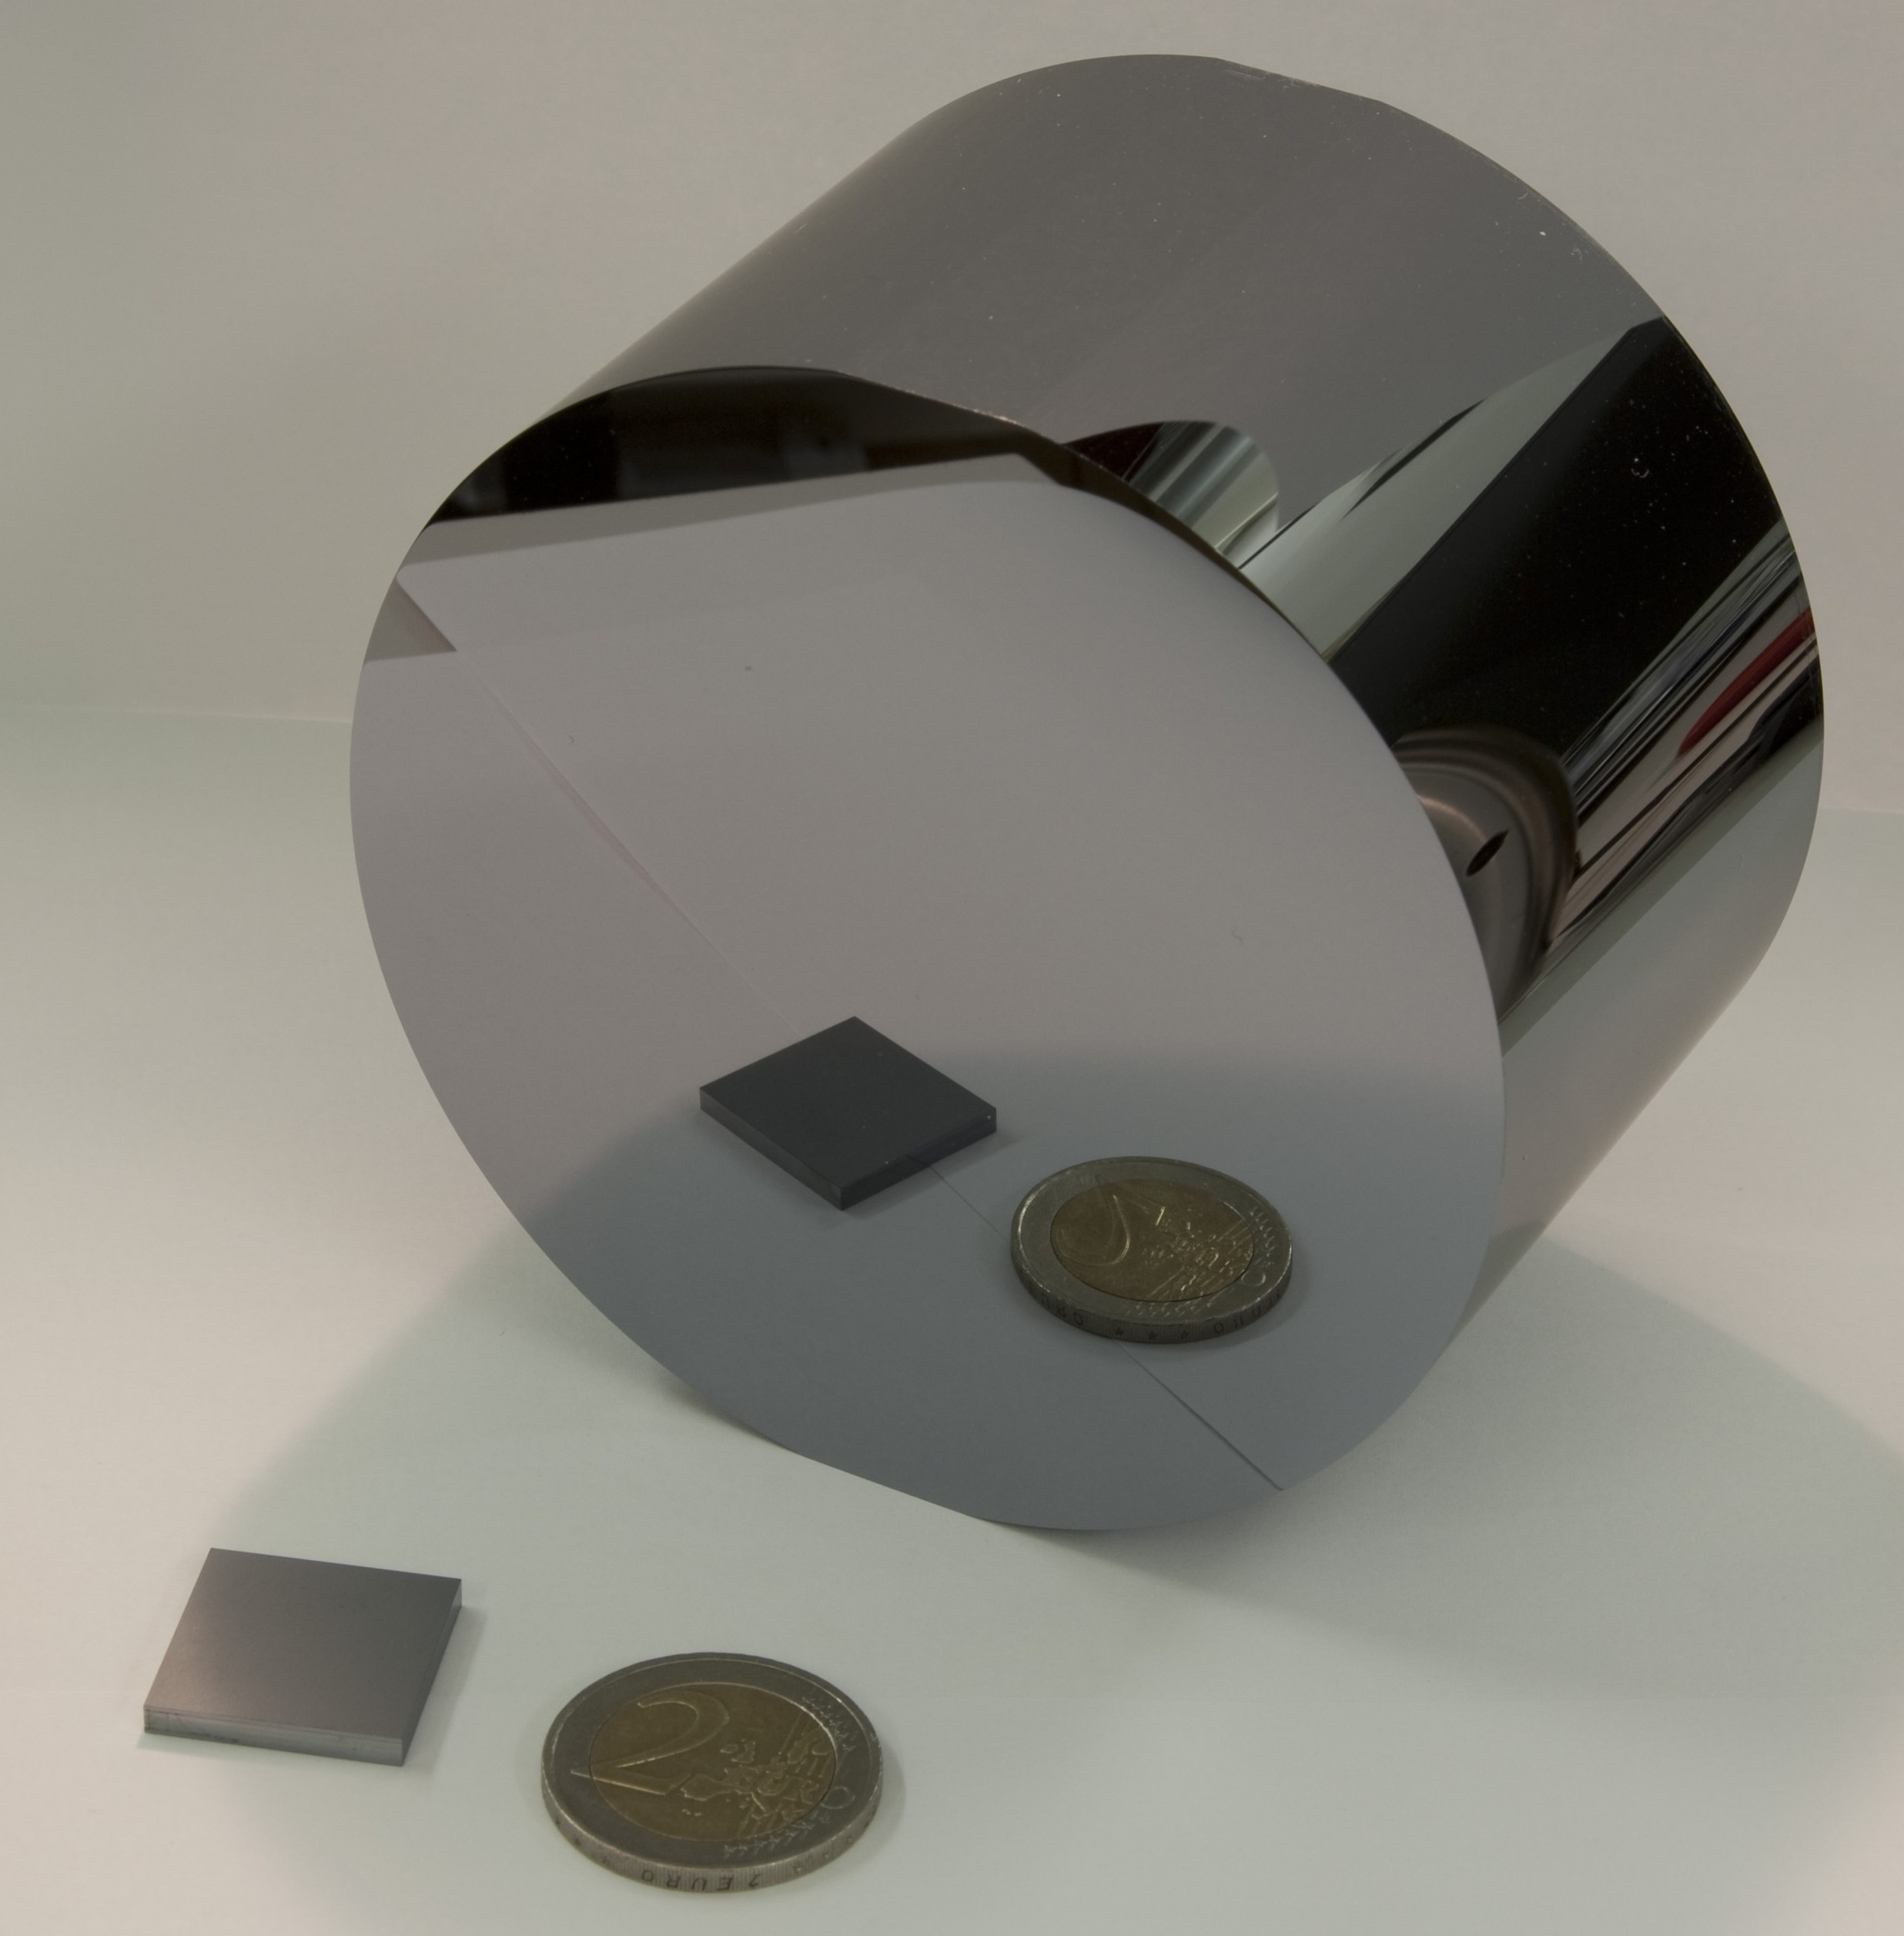
\includegraphics[width=0.49\linewidth]{Sec_Optics/Si_bulk.jpg}
\caption{Silicon sample as being used for cryogenic mechanical loss measurements \cite{Nawrodt2008}. The single crystalline material is cut in a cylindrical shape and polished at the front and back side as well as the barrel.}
\label{fig:si_pic}
\end{center}
\end{figure}

Due to the huge demand of high purity silicon wafers for the semiconductor industry silicon bulk samples are available in relative large pieces. The available sample diameter is dependent on the fabrication process. The two main growing processes for single crystal silicon used in semiconductor industry are the Czochralski (CZ) and the Float Zone (FZ) method. CZ silicon is grown from a silicon melt in a silica crucible. It results in relative large samples with a reasonable purity. The most dominant impurities in undoped CZ-grown silicon are carbon (typically $10^{18}\,\mathrm{cm}^{-3}$) and oxygen (typically up to $10^{19}\,\mathrm{cm}^{-3}$). In contrast, FZ silicon contains these impurities typically with much smaller concentrations (up to $10^3$ times smaller). Single or poly-crystalline silicon is remelt by means of inductive heating in vacuum or under an inert atmosphere during the FZ process. Impurities dissolve better in the melt than in the solid part. The re-crystallised material has therefore a higher purity than the initial one. By slowly sweeping the melt from one end to the other it is possible to purify in steps. The mechanism of inductive heating sets limits to the currently available setups and leads to smaller currently available samples\footnote{There is still no technical limit reached for the float zone process. The maximum diameter currently available is set by the demands of the semiconductor market.}. Well established polishing methods exist for silicon due to the wafer fabrication. Micro roughness and flatness needed for optical applications can be achieved. Additionally, silicon provides the possibility of jointing pieces by means of bonding techniques (see also section~\ref{sec:technologies}). Two possible techniques under discussion are anodic bonding and the well establish hydroxide catalysis bonding~\cite{Veggel2009,Dari2010} currently in use in 1st and 2nd generation detectors. 

Using silicon as a test mass material demands a change in operational wavelength. Silicon is not transparent at 1064\,nm (optical absorption is approximately $10^{-1}\,cm^{-1}$ at 1064\,nm \cite{Green1995}), and has a smaller optical absorption at longer wavelengths. Erbium-fibre lasers provide a reliable light source in the IR spectrum. At 1550\,nm silicon is transparent and can be used as an standard optical material in reflection and transmission applications. Optical absorption measurements based on the creation of electron-hole-pairs suggests a minimum absorption of $3.2\times10^{-2}\,cm^{-1}$ at 1450\,nm at room temperature~\cite{Keevers1995}. However, a detailed analysis of the absorption processes and the total optical absorption of silicon at 1550\,nm and low temperatures does not exist so far. A similar lack of parameters exists for other optical properties like the refraction index $n$ or the thermo-refractive coefficient $dn/dT$~\cite{Frey2006}. Currently, several institutions wor ldwide are investigating these optical properties. Several institutions involved in this design study play a key role in this research.
 
A collection of the mechanical and thermal properties of fused silica, sapphire and silicon can be found in appendix~\ref{app:mechdat} and appendix~\ref{app:thermdat}. Selected literature values at 10, 20, 30 and 300\,K have been summarized in table~\ref{tab:tn_T_param} and \ref{tab:tn_param}. These values have been used for all thermal noise estimates presented within this document.
 
\begin{table}[!t]
\begin{center}
\begin{tabular}{|l|c|c|c|c|c|c|c|} \hline
\multirow{2}{*}{Parameter} & \multirow{2}{*}{T} & \multicolumn{2}{c|}{Fused silica} & \multicolumn{2}{c|}{Sapphire} & \multicolumn{2}{c|}{Silicon} \\ 
					    &        & Value & Ref. & Value & Ref. & Value & Ref. \\ \hline
 				      & 10\,K  & 6.3 & \cite{Touloukian1970_Cp_nonmetal} & 0.085 & \cite{White1994} & 0.276 & \cite{Hull1999} \\
heat capacity & 20\,K  & 25.2 & \cite{Touloukian1970_Cp_nonmetal} & 0.72 & \cite{White1994} & 3.41 & \cite{Hull1999}  \\
(J/kg\,K)     & 30\,K  & 54.6 & \cite{Touloukian1970_Cp_nonmetal} & 2.6 & \cite{White1994} & 18.55 & \cite{Hull1999} \\ 
						  & 300\,K & 738 & \cite{Touloukian1970_Cp_nonmetal} & 781 & \cite{White1994} & 713 & \cite{Hull1999} \\ \hline
     					& 10\,K & 0.098 & \cite{Touloukian1970_kappa_nonmetal} & 2900 & \cite{Touloukian1970_kappa_nonmetal} & 2110 & \cite{Touloukian1970_kappa_metal} \\ 
thermal conductivity  & 20\,K  & 0.13 & \cite{Touloukian1970_kappa_nonmetal} & 15700 & \cite{Touloukian1970_kappa_nonmetal} & 4940 & \cite{Touloukian1970_kappa_metal}  \\ 					  
(W/m\,K)  		& 30\,K & 0.18 & \cite{Touloukian1970_kappa_nonmetal} & 20700  & \cite{Touloukian1970_kappa_nonmetal} & 4810 & \cite{Touloukian1970_kappa_metal} \\ 
							& 300\,K & 1.5 & \cite{Touloukian1970_kappa_nonmetal} & 46 & \cite{Touloukian1970_kappa_nonmetal} & 148 & \cite{Touloukian1970_kappa_metal} \\ \hline
thermal expansion & 10\,K & $\mathrm{-2.2\times10^{-7}} $ & \cite{Touloukian1970_alpha_nonmetal} & $\mathrm{1.0\times10^{-9}}$ & \cite{White1994} & $\mathrm{8.8\times10^{-10}} $ & \cite{Hull1999} \\ 
coefficient		& 20\,K  & $\mathrm{-5.8\times10^{-7}} $ & \cite{Touloukian1970_alpha_nonmetal} & $\mathrm{4.0\times10^{-9}}$ & \cite{White1994} & $\mathrm{-2.5\times10^{-9}} $ & \cite{Hull1999}  \\ 
(1/K)        	& 30\,K  & $\mathrm{-8.0\times10^{-7}} $ & \cite{Touloukian1970_alpha_nonmetal} & $\mathrm{1.6\times10^{-8}}$ & \cite{White1994} & $\mathrm{-5.3\times10^{-8}} $ & \cite{Hull1999} \\ 							
							& 300\,K & $\mathrm{5.0\times10^{-10}} $ & \cite{Touloukian1970_alpha_nonmetal} & $\mathrm{5.6\times10^{-6}}$ & \cite{White1994} & $\mathrm{2.7\times10^{-6}} $ & \cite{Hull1999} \\ \hline
\multirow{4}{*}{mechanical loss} & 10\,K & $\mathrm{7.9\times10^{-4}} $ & \cite{Schwarz2009} & $\mathrm{5\times10^{-9}}$ & \cite{Uchiyama1999} & $\mathrm{1\times10^{-9}}$ & \cite{McGuigan1978}\\
							& 20\,K & $\mathrm{1.0\times10^{-3}} $ & \cite{Schwarz2009} & $\mathrm{5.6\times10^{-9}}$ & \cite{Uchiyama1999} & $\mathrm{4\times10^{-9}}$ & \cite{Nawrodt2008}\\
 							& 30\,K & $\mathrm{1.0\times10^{-3}} $ & \cite{Schwarz2009} & $\mathrm{1.4\times10^{-8}}$ & \cite{Uchiyama1999} & $\mathrm{5\times10^{-9}}$ & \cite{McGuigan1978}\\							
							& 300\,K & $\mathrm{4\times10^{-10}} $ & \cite{Penn2006} & $\mathrm{3.8\times10^{-9}} $ & \cite{Rowan2000} & $\mathrm{1\times10^{-8}}$ & \cite{Nawrodt2008} \\ \hline
\multirow{4}{*}{$dn/dT$ (1/K)} & 10\,K & -- & -- & $\mathrm{<9\times10^{-8}} $ & \cite{Tomaru2002a} & $\mathit{<1\times10^{-6}} $ & -- \\
							& 20\,K & -- & -- & $\mathrm{<9\times10^{-8}} $ & \cite{Tomaru2002a} & $\mathrm{1\times10^{-6}}$ & -- \\
							& 30\,K & $\mathrm{1\times10^{-6}}$ & \cite{Leviton2006} & $\mathrm{<9\times10^{-8}} $ & \cite{Tomaru2002a} & $\mathrm{3.3\times10^{-6}}$ &\cite{Frey2006}\\									
							& 300\,K & $\mathrm{8\times10^{-6}}$ & \cite{Leviton2006} & $\mathrm{1.3\times10^{-5}}$ & \cite{Malitson1962} & $\mathrm{1.9\times10^{-4}}$& \cite{Frey2006} \\ \hline
\end{tabular}
\end{center}
\caption{Temperature dependent thermal parameters for fused silica, sapphire and silicon bulk material used for thermal noise estimates at selected temperatures. $dn/dT$ is given at 1064\,nm for fused silica and sapphire and at 1550\,nm for silicon.}
\label{tab:tn_T_param}
\end{table}

\begin{table}
\begin{center}
\begin{tabular}{|l|c|c|c|c|c|c|} \hline
\multirow{2}{*}{Parameter} & \multicolumn{2}{c|}{Fused silica} & \multicolumn{2}{c|}{Sapphire} & \multicolumn{2}{c|}{Silicon} \\ 
					    & Value & Ref. & Value & Ref. & Value & Ref. \\ \hline
density $\rho$ ($\mathrm{kg/m^3}$) & 2202 & \cite{Nawrodt2009_ET} & 3980 & \cite{Nawrodt2009_ET} & 2330 & \cite{Nawrodt2009_ET} \\ 
Young's modulus $Y$ (GPa)& 72 & \cite{Nawrodt2009_ET} & 400 & \cite{Nawrodt2009_ET} & 188 & \cite{Nawrodt2009_ET} \\
Poisson's ratio $\nu$ & 0.17 & \cite{Nawrodt2009_ET} & 0.24 & \cite{MPDB} & 0.22 & \cite{Nawrodt2009_ET}  \\ 
refractive index $n$ & 1.45 & \cite{Franc2009} & 1.75 & \cite{Franc2009} & 3.453 & \cite{Franc2009} \\
\hline
\end{tabular}
\end{center}
\caption{Parameters of bulk materials that are assumed to be temperature independent for the thermal noise calculations. The refractive index of fused silica and sapphire is given at 1064\,nm whereas this parameter is listed at 1550\,nm for silicon.}
\label{tab:tn_param}
\end{table}

\FloatBarrier
\subsubsection{Coating material selection}
%\emph{Author: J. Franc}

The construction of the 3rd generation of GW detectors has specific constraints on the thermal noise level. Several studies have already demonstrated that the coating is the most important noise source in the frequency range around 10 to 100\,Hz. To avoid coating materials generating a noise level larger than the expected sensitivity, very high quality coatings are needed. First, the absorption has to be less than 5\,ppm and the loss angle of the material has to be as low as possible in order to obtain a minimum coating Brownian noise level. To produce coatings with such quality, an ion beam sputtering is needed. Mirrors for GW detectors involve several parameters: the nature of the substrate (polishing, operational temperature), the characteristic of the sputtering source in the coater (temperature and emission law) and the pressure in the coater. To get a coating that follows the GW detector specifications, sputtering deposition is required because the energy lies in the range of 10 to 50\,eV and the impact velocity is in the range of km/s \cite{Mackowski2005}. This causes a dense coating with a high optical and mechanical quality.
 
Driven by the research performed for the 1st and 2nd generation of GW detectors, a state-of-the-art deposition technique - ion-beam-sputtering (see box~\ref{box:IBS}) exists that provides high performances coatings.

\longetbox{i}{box:IBS}{Ion Beam Sputtering}{Coatings for the current GW detectors are made by an ion-beam-sputtering (IBS) technique. The target material is hit by accelerated ions (typically argon ions) coming from an ion source. This source consists of a heated cathode and an anode which are arranged along a common axis. Applying a high voltage between the anode and cathode creates an electrical field inside the ion source, confining electrons from the heated cathode in the center of the source. When argon is injected into the source the high electric field causes the gas to ionize - a plasma is created inside the source. The positively charged argon ions are accelerated by means of the high electric field inside the source towards the cathode forming a collimated ion beam. This ion beam is pointed towards the sputtering target where it sputters the target material onto the sample.
\begin{figure}[H]
\begin{center}
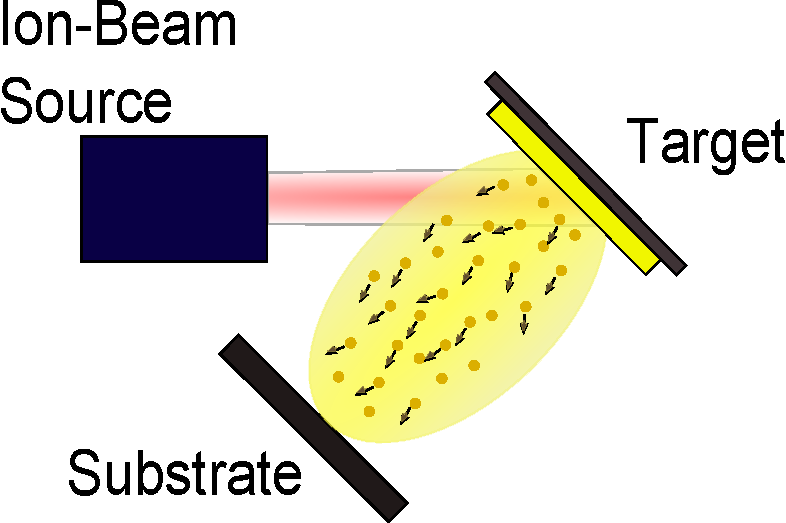
\includegraphics[width=0.4\linewidth]{Sec_Optics/IBS.pdf}
\vspace{3mm}
\caption{Schematic view of an ion-beam-sputtering process. Ions are created and accelerated inside the ion source. The ion beam is pointed towards the target where it releases the sputtering material. This material is deposit on the substrate forming a dense coating.}
\end{center}
\end{figure}
The high energy of the argon ions allows a good transfer of energy and momentum on the target particles. Thus, the coating material particles arrive with a high energy and momentum at the substrate forming a very dense and homogeneous coating. It has been shown in the past that IBS creates coatings with the lowest mechanical loss among all other coating techniques (e.g. magnetron sputtering, electron beam vapour deposition, etc.). Thus, IBS is currently the best technology to create high performance optical coatings.
\begin{figure}[H]
\begin{center}
\subfigure[]{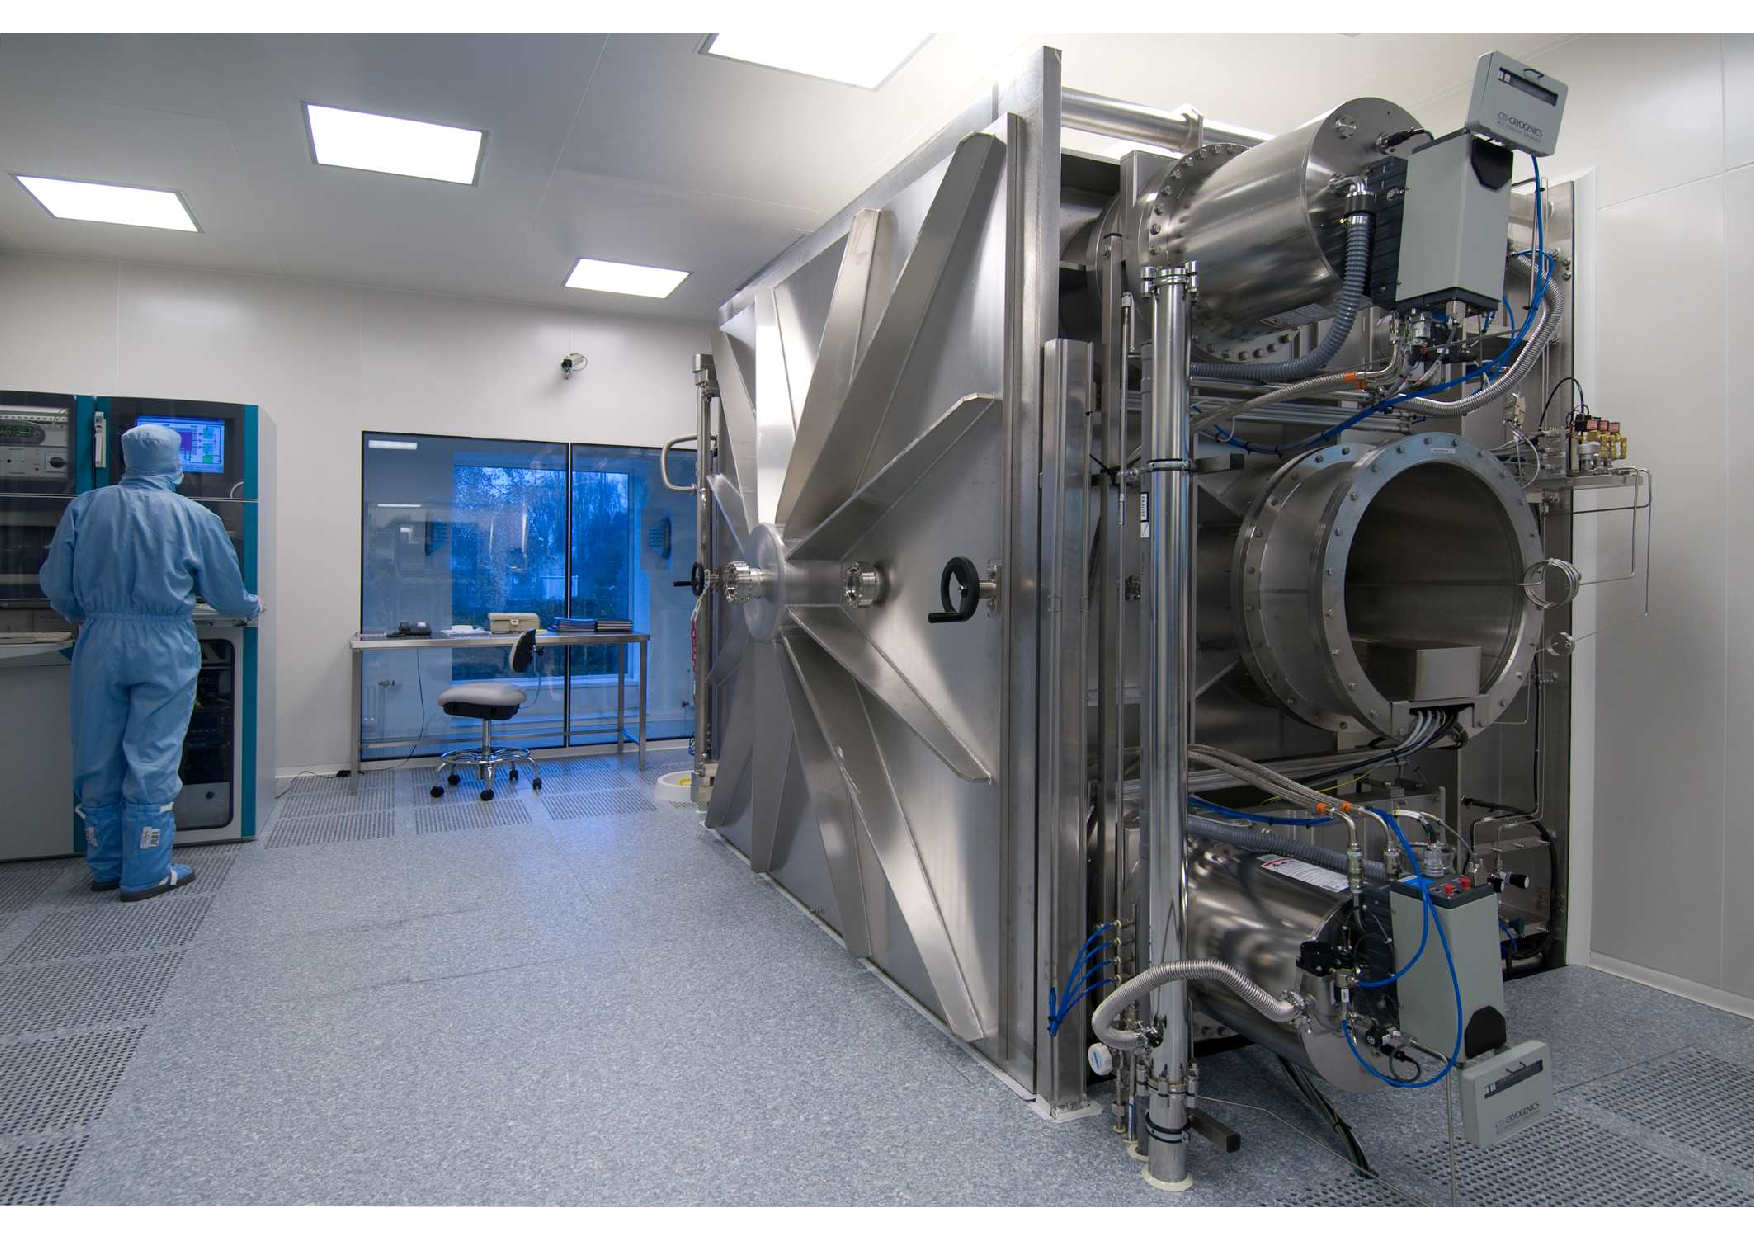
\includegraphics[width=0.49\linewidth]{Sec_Optics/coater1.pdf}}
\subfigure[]{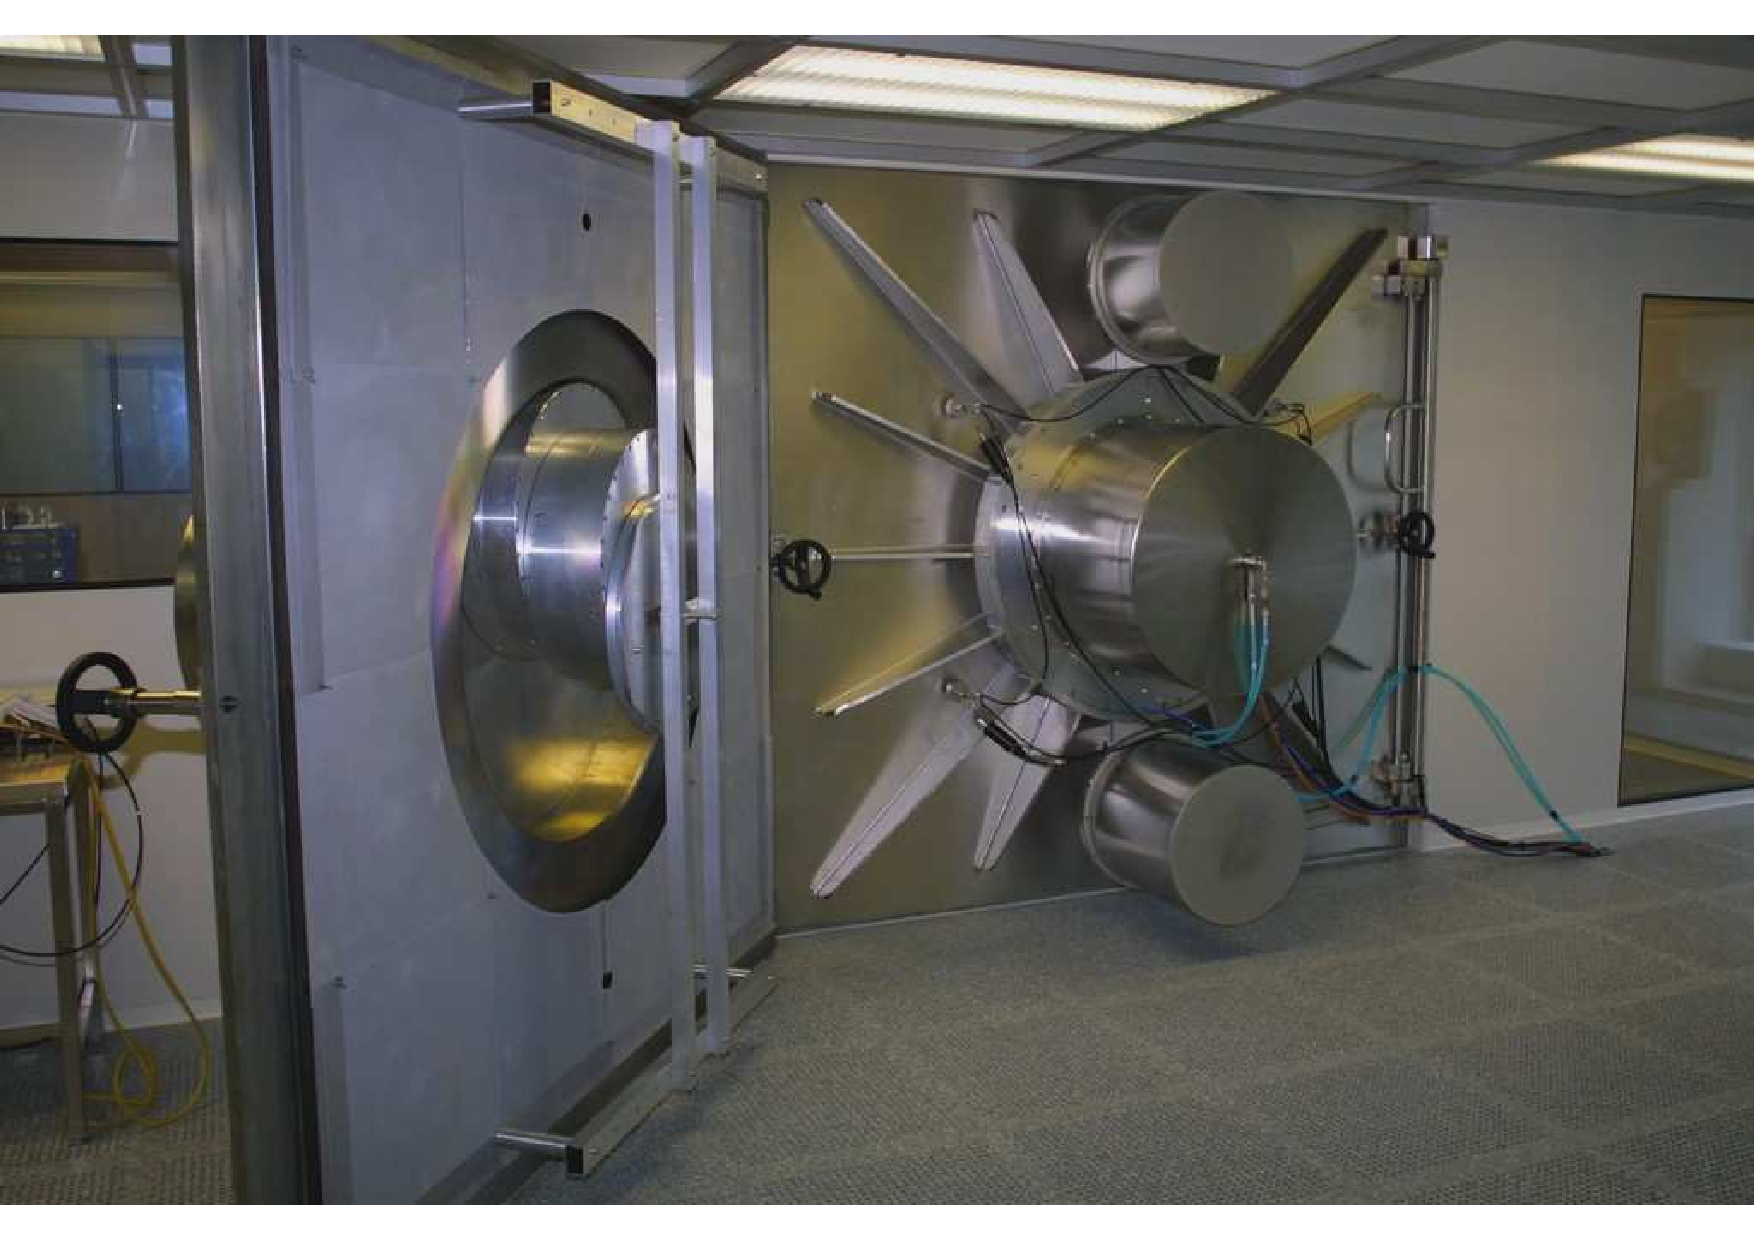
\includegraphics[width=0.49\linewidth]{Sec_Optics/coater2.pdf}}
\caption{IBS coating machines operated at the Laboratoire des Mat\'eriaux Avanc\'es (LMA) in Lyon.}
\end{center}
\end{figure}
The world largest IBS coater is currently operated at the Laboratoire des Mat\'eriaux Avanc\'es (LMA) in Lyon. The vacuum chamber has a size of 2.4 x 2.4 x 2.2 $\mathrm{m^3}$ which allows the fabrication of coatings for current and future GW detectors. The coating machine is operated in a class 1 clean room to fulfill the requirements of high performance optics. This coating machine would be capable of fabrication the mirrors for the proposed Einstein Telescope based on silica and tantala.
}


Typically, $\lambda/4$ layers of alternating low and high refractive index materials are used to form a high-reflectivity coating. Commonly used materials are tantala ($\mathrm{Ta_2O_5}$) as the high refractive index material and silica ($\mathrm{SiO_2}$) as the low refractive index material.

At first, the design study considered silica (refractive index n=1.45) and tantala (refractive index n=2.03). These two materials' oxide layers have the best optical and mechanical properties in the 1st and 2nd generation of GW detectors. The measurements made on the $\mathrm{Ta_2O_5/SiO_2}$ coatings have shown that the lossier material is the $\mathrm{Ta_2O_5}$. Thus, the material improvement has been focused on tantala. Several doped materials were tested to improve the mechanical losses of $\mathrm{Ta_2O_5}$. By doping $\mathrm{Ta_2O_5}$ with Ti and with an optimization of the deposition process, it is possible to decrease the losses of high refractive index material from $3.8\times10^{-4}$ to $2\times10^{-4}$. To date, other materials have been considered for doping the $\mathrm{Ta_2O_5}$ layers. New materials should also be considered to replace the $\mathrm{Ta_2O_5}$ layers with another high refractive index material. In this context, table~\ref{tab:Coat_param} presents the parameters values needed for thermal noise calculation for different coating materials. A summary of the thermal noise estimates can be found in~\cite{Franc2009,Nawrodt2009_ET}.

%\begin{turn}{90}
\begin{sidewaystable}
%\begin{table}
\begin{center}
\begin{tabular}{|l|c|c|c|c|c|c|c|}
\hline
& $\mathrm{SiO_2}$ & $\mathrm{Al_2O_3}$ & $\mathrm{Ti:Ta_2O_5}$ & $\mathrm{Ta_2O_5}$ & $\mathrm{TiO_2}$ & $\mathrm{Nb_2O_5}$ & $\mathrm{ZrO_2}$\\
\hline
Loss angle & $0.5\times10^{-4}$ & $2.4\times10^{-4}$ & $2\times10^{-4}$ & $3.8\times10^{-4}$ & $6.3\times10^{-3}$ & $6.7\times10^{-4}$ & $2.85\times10^{-4}$\\
Density ($\mathrm{kg\,m^{-3}}$) & 2200 & 3700 & 6425 & 6850 & 4230 & 4590 & 6000 \\
Thermal conductivity ($\mathrm{W\,m^{-1}\,K^{-1}}$) & 0.5 & 3.3 & 0.6 & 0.6 & 0.45 & 1 & 1.09 \\ 
Specific heat ($\mathrm{J\,K^{-1}\, kg^{-1}}$) & 746 & 310 & 269 & 306 & 130 & 590 & 26 \\
Thermal expansion coefficient ($\mathrm{K^{-1}}$) & $0.51\times10^{-6}$ & $8.4\times10^{-6}$ & $3.6\times10^{-6}$ & $3.6\times10^{-6}$ & $5\times10^{-5}$ & $5.8\times10^{-6}$ & $10.3\times10^{-6}$ \\
Thermo-optic coefficient ($\mathrm{K^{-1}}$) & $8\times10^{-6}$ & $1.3\times10^{-5}$ & $14\times10^{-6}$ & $2.3\times10^{-6}$ & $-1.8\times10^{-4}$ & $1.43\times10^{-5}$ & $10\times10^{-5}$\\
Young's modulus (GPa) & 60 & 210 & 140 & 140 & 290 & 60 & 200 \\
Poisson's ratio & 0.17 & 0.22 & 0.23 & 0.23 & 0.28 & 0.2 & 0.27 \\
Refractive index & 1.45 & 1.63 & 2.06 & 2.03 & 2.3 & 2.21 & 2.15 \\
\hline
\end{tabular}
\end{center}
\caption{List of the optical and mechanical values of different coating materials at 300\,K.}
\label{tab:Coat_param}
%\end{table}
\end{sidewaystable}
%\end{turn}

%\emph{Author: I. Martin}

Extensive studies of the temperature dependence of the mechanical loss of tantala ($\mathrm{Ta_2O_5}$) have been undertaken and the effects of post-deposition heat-treatment and of doping with titania ($\mathrm{TiO_2}$) have been investigated~\cite{Martin2008,Martin2009,Martin2010}. In general the loss increases at low temperature, with three loss peaks observed to occur at different heat-treatment temperatures. Tantala heat-treated at 300$\mathrm{^\circ}$C and 400$\mathrm{^\circ}$C exhibits a loss peak at approximately 35\,K. A larger and narrower loss peak was observed at 20\,K in tantala coatings heat-treated at 600$\mathrm{^\circ}$C. There is some evidence that the 35\,K peak may also be present in tantala heat-treated at 600$\mathrm{^\circ}$C, underlying the peak at 20\,K. It is known that ion-beam sputtered tantala crystallises when heated above approximately 650$\mathrm{^\circ}$C. A large and very broad loss peak has been observed in tantala heat-treated at 800$\mathrm{^\circ}$C. 
While of interest for studies of the loss mechanisms in tantala, crystallised tantala is not suitable for use in an high-reflective coating due to its poor optical properties.

\begin{figure}[!h]
\begin{center}
\subfigure[]{\includegraphics[width=0.49\linewidth]{Sec_Optics/coat_anneal.pdf}}
\subfigure[]{\includegraphics[width=0.49\linewidth]{Sec_Optics/silica_tantala_loss.pdf}}
\end{center}
\caption{(a)~--~Measured values of the coating loss of tantala annealed at different temperatures. (b)~--~Comparison of 600$\mathrm{^\circ}$C heat treated tantala and silica coatings at low temperatures and 350\,Hz.}
\label{fig:coating_loss_cryo}
\end{figure}

Further work may be required to establish the optimum heat-treatment temperature for a silica/tantala multilayer coating for use at cryogenic temperature. High heat-treatment temperatures are generally desirable for optimal optical properties. Furthermore, studies of the mechanical loss of ion-beam sputtered silica coatings have shown a systematic reduction in the loss at room temperature with increasing heat-treatment temperatures. Thus carrying out heat-treatment at the maximum temperature which can be achieved without inducing crystallisation in the tantala layers may be desirable. However, as shown in Figure~\ref{fig:coating_loss_cryo}(a), tantala has a significantly lower loss at temperatures below 100\,K when heat-treated at lower temperatures (300 or 400$\mathrm{^\circ}$C) than when heat-treated at 600$\mathrm{^\circ}$C. While the loss of the tantala layers dominate the loss of a multilayer silica/tantala coating at room temperature, the loss of ion-beam sputtered silica has a similar magnitude as the loss of tantala at temperatures below 50\,K. Thus further studies of the effect of heat-treatment on the temperature dependence of the mechanical loss of ion-beam sputtered silica are also required to allow the optimal heat-treatment temperature to be chosen. In addition, measurements of the temperature dependence of the optical properties of the coating may be required.

A comprehensive summary of R\&D activites needed for understanding and characterising the coating properties can be found in section~\ref{sec:coating_RND}.

\FloatBarrier
\subsubsection{Thermal noise estimates for reflective components}
\label{sec:TN_refl}

%\emph{Author: R. Nawrodt}

The thermal noise of a fully reflective mirror comprises thermal noise arising from the bulk material and the coating. The bulk material thermal noise consists of Brownian thermal noise and thermo-elastic noise. Brownian noise represents the thermal fluctuations (`Brownian motion') of the atoms within the bulk material and is dependent on the sample temperature $T$ and the mechanical loss of the bulk material $\phi$ \cite{Harry2002,Harry2006}:

\begin{equation}
S_\mathrm{x}^\mathrm{bulk}(f,T) = 2k_\mathrm{B}T\frac{1-\nu}{\pi^{3/2}fYw}\phi
\label{eq:bulk_Brownian}
\end{equation} 

with the Boltzmann constant $k_\mathrm{B}$, the frequency $f$, the beam radius $w$, the substrate Poisson's ratio $\nu$ and Young's modulus $Y$. It is obvious that the Brownian thermal noise is only dependent on mechanical properties of the material.

\longetbox{i}{box:TN}{Thermal noise in optical components}{There are two fundamental origins of thermal noise in optical components: The first is driven by the thermal energy $k_\mathrm{B}T$ that is present as soon as the component is operated at non-zero temperatures. Here, the thermal energy causes thermal fluctuations of the atoms of the optical component, which causes a thermally driven fluctuation of the reflective surface of the element. This type of noise is probably closest to the process that to mind when talking about thermal noise. In many different field this type of noise---Brownian noise---is present. Throughout this document this type of noise is called Brownian thermal noise.\\
However, there is a second type of noise that arises from temperature fluctuations. When operating a macroscopic object at non-zero temperatures the local (microscopic) temperature is not a constant value but fluctuates around the average temperature~$T$. Due to the fact that many material properties are temperature dependent this opens a channel to introduce the second type of noise. Here, the temperature fluctuation causes a phase or position fluctuation by means of the temperature dependence of a property, e.g.\ the coefficient of thermal expansion~$\alpha$ or the refractive index~$n$. The process that is associated with $\alpha$ is called thermo-elastic noise whereas the other process is referred to as thermo-refractive noise.\\
Although in both cases the temperature is the fundamental driving force one distinguishes between then strictly due to the different coupling mechanisms of the fluctuation to the read-out noise.}

The thermo-elastic noise of the bulk material is created by statistical temperature fluctuations. By means of the coefficient of thermal expansion $\alpha$ these fluctuations are translated into displacement noise. The thermo-elastic spectral noise density is given by~\cite{Braginsky1999a}:

\begin{equation}
S_\mathrm{TE}^\mathrm{bulk}(f,T) = \frac{4k_\mathrm{B}T^2\alpha^2(1+\nu)^2\kappa}{\sqrt{\pi^5}\rho^2C^2f^2w^3}
\label{eq:bulk_TE}
\end{equation}

with the coefficient of thermal expansion $\alpha$, the thermal conductivity $\kappa$, the heat capacity $C$, and the mass density $\rho$. This equation is valid if the thermal diffusion length 

\begin{equation}
l_\mathrm{th} = \sqrt{\frac{a^2}{f}}
\end{equation}

of the material is smaller than the beam diameter. The parameter $a^2 = \kappa/(\rho C)$. This assumption is called the adiabatic case. During one period of oscillation all temperature fluctuations that are present at the observation volume stay inside this volume. If the thermal diffusion length gets larger (e.g.\ by means of high thermal conductivity or low frequencies) the thermo-elastic effect gets weaker. Especially, for low temperature applications this non-adiabatic correction becomes important and reduces the contribution of thermo-elastic noise further. This correction has been taken into account for all calculations presented in this document. Details of the calculation can be found in~\cite{Cerdonio2001,Nawrodt2009_ET}.

Figure~\ref{fig:bulk_TN} compares the Brownian and thermo-elastic noise of one single mirror made of fused silica, sapphire or silicon at 10 and 300\,K. The parameters used for the calculation are listed in tables~\ref{tab:tn_T_param} and \ref{tab:tn_param}.

\begin{figure}
\begin{center}
\subfigure[]{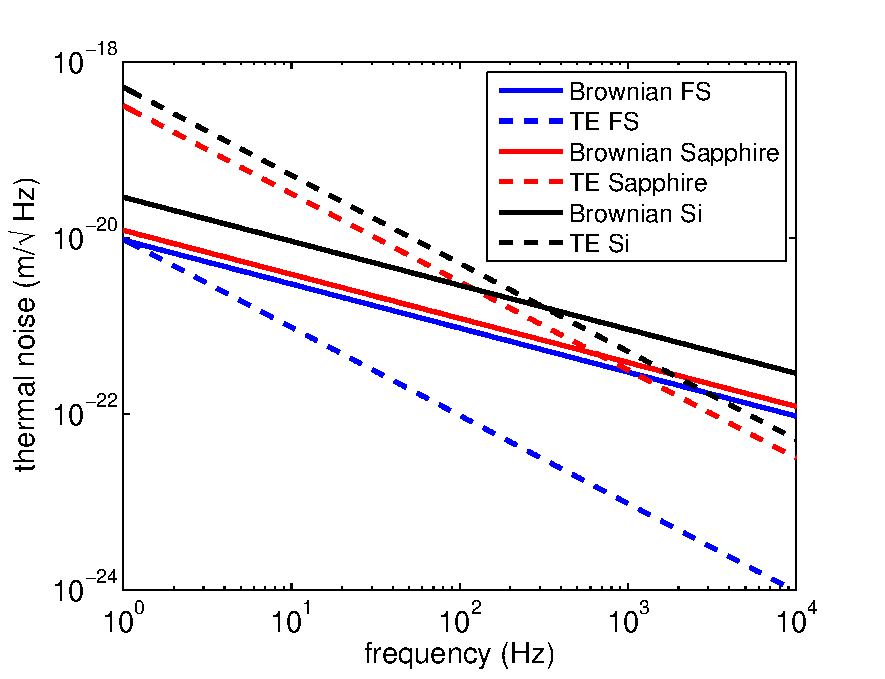
\includegraphics[width=0.49\linewidth]{Sec_Optics/bulk_TN_300K.pdf}}
\subfigure[]{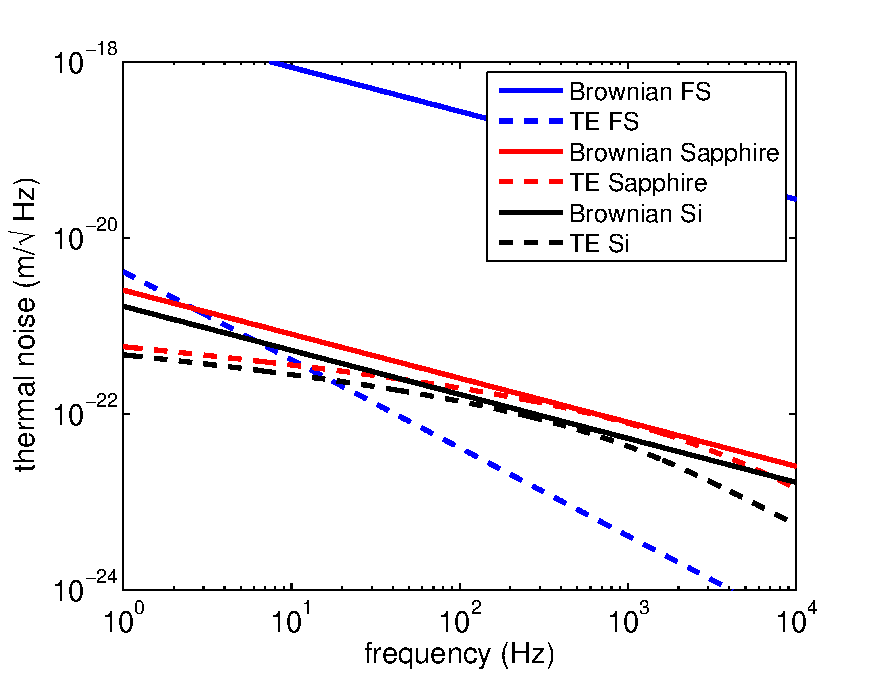
\includegraphics[width=0.49\linewidth]{Sec_Optics/bulk_TN_10K.pdf}}
\end{center}
\caption{Comparison of the Brownian and thermo-elastic noise for fused silica, sapphire and silicon at 300\,K~(a) and 10\,K~(b) (TE~--~thermo-elastic noise, FS~--~fused silica). At room temperature the crystalline substrate materials show a large thermo-elastic noise. In contrast, at cryogenic temperatures fused silica has a large Brownian thermal noise due to its large mechanical loss.}
\label{fig:bulk_TN}
\end{figure}

At room temperature fused silica provides the lowest level of thermal noise due to its low mechanical loss and small coefficient of thermal expansion (see figure~\ref{fig:bulk_TN}(a)). All crystalline materials show a high coefficient of thermal expansion and thus a large thermo-elastic noise. Therefore, crystalline materials should be avoided in room temperature detectors in order to achieve the minimum thermal noise level of a mirror substrate.

In contrast, at low temperatures fused silica has a large mechanical loss reaching values of $10^{-3}$ around 10\,K. Crystalline materials behave differently resulting in a low mechanical loss of better than $10^{-8}$ at low temperatures (see Tab.~\ref{tab:tn_T_param}). Additionally, the coefficient of thermal expansion is very small at low temperatures. This reduces dramatically the thermo-elastic noise contribution compared to room temperature operation (see figure~\ref{fig:bulk_TN}(b)). Thus, using cryogenic temperatures and crystalline materials will result in a low total bulk thermal noise.

\begin{figure}[!h]
\begin{center}
\subfigure[]{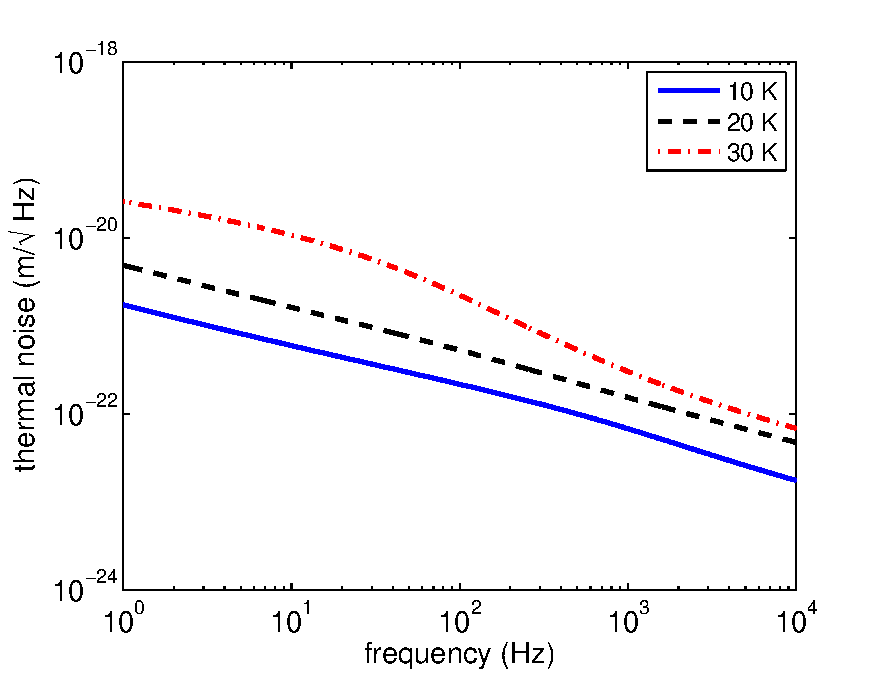
\includegraphics[width=0.49\linewidth]{Sec_Optics/bulk_Si_comp.pdf}}
\subfigure[]{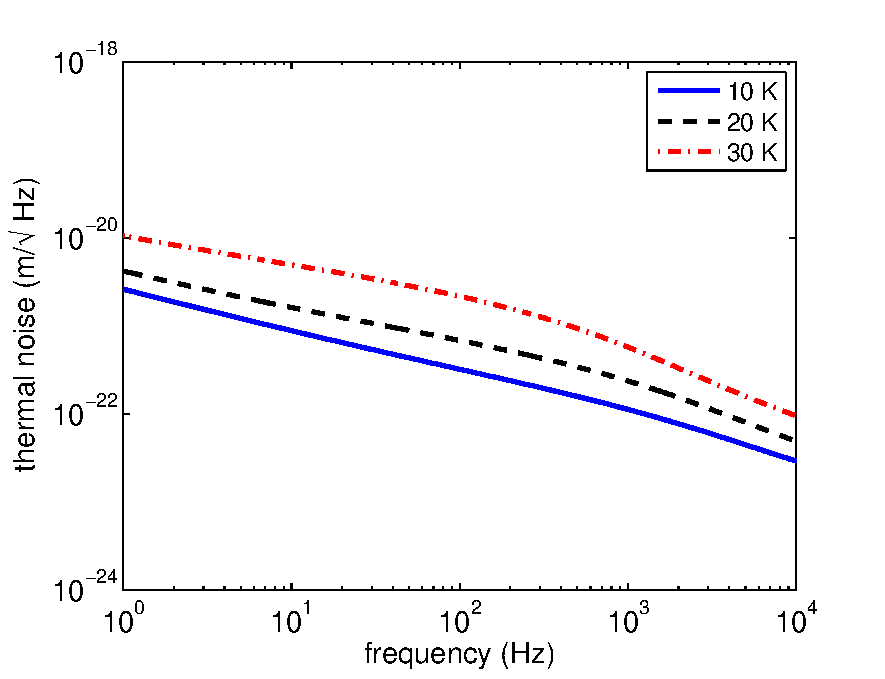
\includegraphics[width=0.49\linewidth]{Sec_Optics/bulk_Sapphire_comp.pdf}}
\end{center}
\caption{Comparison of the total bulk thermal noise of a mirror substrate made of silicon~(a) and sapphire~(b) at different temperatures. The parameters used for this calculation are summarised in tables~\ref{tab:tn_T_param} and \ref{tab:tn_param}.}
\label{fig:bulk_T_TN}
\end{figure}

Figure~\ref{fig:bulk_T_TN} compares the total bulk thermal-noise consisting of thermo-elastic and Brownian thermal noise for sapphire and silicon at selected temperatures. Due to the small mechanical loss and coefficient of thermal expansion, a low thermal noise level is achieved. At 20\,K both materials show a comparable thermal noise level. At higher temperatures thermo-elastic noise becomes dominant. Here, sapphire has a slightly lower level of thermo-elastic noise due to the combination of its thermal properties (mainly the high thermal conductivity). At 10\,K silicon has a slightly lower total thermal noise than a sapphire mirror substrate. 

All calculations so far are based on semi-infinite mirror substrates. This assumption is true for a first comparison of the materials and in cases where the beam radius compared to the mirror radius is small. However, for application in gravitational wave detectors it is preferable to increase the beam diameter to the maximum possible size that is in agreement with the optical clipping losses. The corrections for finite size test masses have been made by different authors for the different noise contributions. The calculations are quite long and thus only the results are shown here. The detailed discussion can be found in the literature \cite{Bondu1998, Liu2000}. 

\begin{figure}[!h]
\begin{center}
\subfigure[]{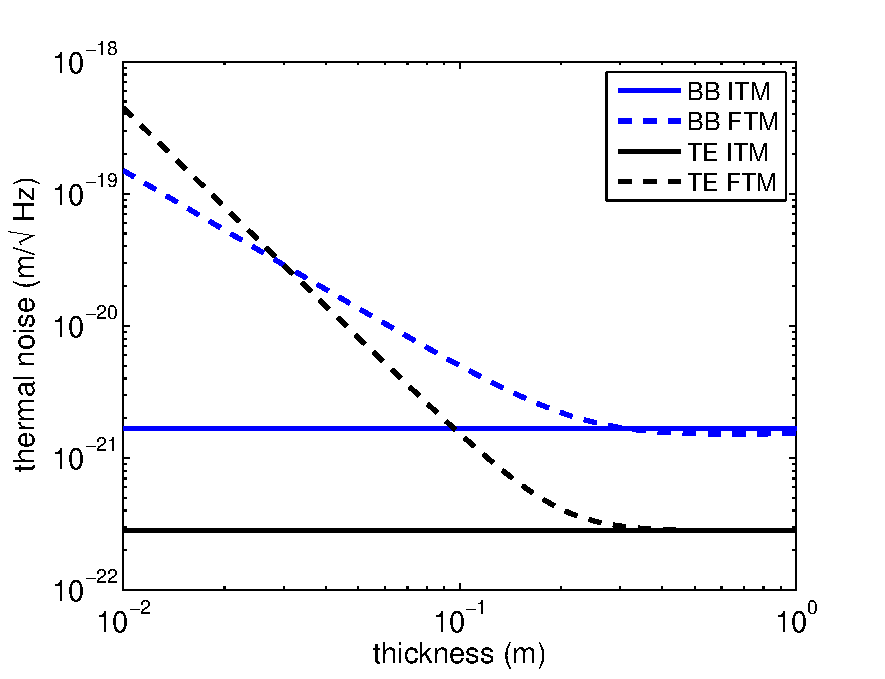
\includegraphics[width=0.49\linewidth]{Sec_Optics/bulk_FTM_thick.pdf}}
\subfigure[]{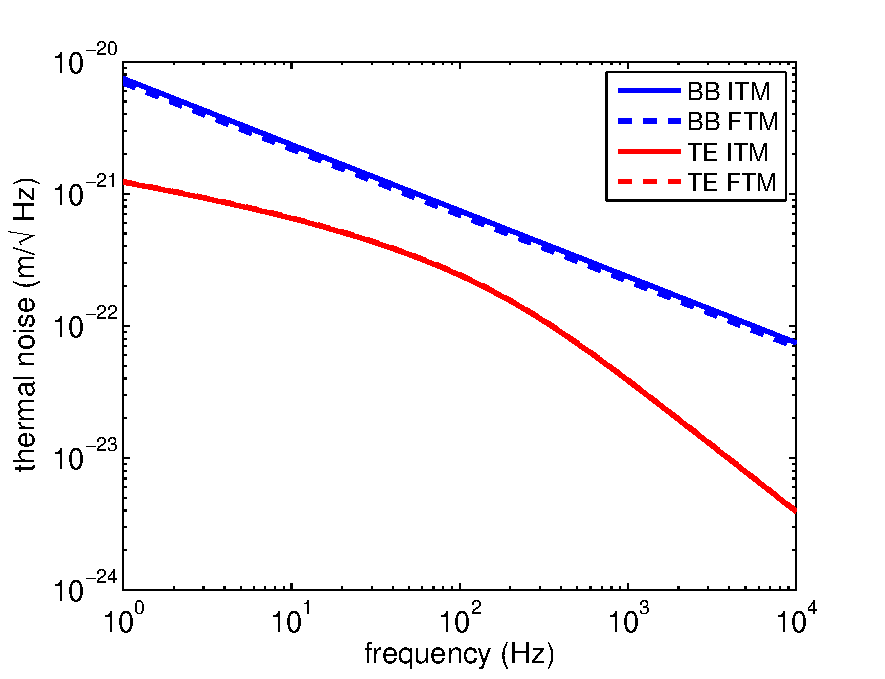
\includegraphics[width=0.49\linewidth]{Sec_Optics/bulk_FTM.pdf}}
\end{center}
\caption{Finite size test mass mirror thermal noise. (a)~--~Dependence of the mirror Brownian and thermo-elastic thermal noise of the thickness of the substrate (silicon, 10\,K, diameter: 0.5\,m, frequency 10\,Hz). (b)~--~Effect of the finite size correction for a typical ET end mirror geometry (silicon, 10\,K). BB~--~bulk Brownian, TE~--~thermo-elastic, ITM~--~inner test mass, ETM~--~end test mass.}
\label{fig:bulk_TN_finite}
\end{figure}

Figure~\ref{fig:bulk_TN_finite} gives the dependence of the substrate thermal noise. It is obvious that for reasonable thicknesses of the substrate the correction is small. Only for very thin substrates does a strong deviation from the simplified infinite half space model appear. At larger thicknesses the finite sample correction leads to a small decrease in thermal noise (approx. $5\dots 10\%$ for bulk Brownian and less than 1\% for bulk thermo-elastic noise).

Optical components being used in GW detectors consist of a bulk material and a coating. The coating usually comprises several alternating dielectric layers formed by high and low refractive index materials. Typically, these layers are formed by amorphous tantala and silica layers with an optical thickness of $\lambda/4$. The circulating laser beam of the interferometer interacts mainly with the coating (point of first contact between light and mirrors). Thus, it can be expected that the optical coating contributes strongly to the total thermal noise of a mirror.

Similar to the thermal noise of the bulk materials, the coatings also show Brownian thermal noise. It is again dependent on the temperature $T$ and the effective mechanical loss $\phi_\mathrm{eff}$ of the coating \cite{Harry2002,Harry2006}:

\begin{equation}
S_x^\mathrm{coating}(f,T) = 2k_\mathrm{B}T\frac{1-\nu}{\pi^{3/2}fYw}\phi_\mathrm{eff}
\label{eq:coat_Brownian}
\end{equation}

with the Boltzmann constant $k_\mathrm{B}$, the frequency $f$, the beam radius $w$, the Poisson's ratio $\nu$ and the Young's modulus $Y$ of the substrate bulk material. The effective mechanical loss contains all coating relevant parameters and is given by:

\begin{equation}
\phi_\mathrm{eff} = \frac{t}{\sqrt{\pi}w}\left(\frac{Y}{Y_\bot}\phi_\bot + \frac{Y_{||}}{Y}\phi_{||} \right).
\label{eq:coat_eff_loss}
\end{equation}

This description of the effective mechanical loss assumes small Poisson's ratios of the coating materials, which is usually fulfilled. $t$ is the total thickness of the coating layer. The Young's moduli $Y_i$, the thicknesses $t_i$ and the mechanical losses $\phi_i$ are combined as follows ($i=1,2$ to indicate the different coating layer properties):

\begin{eqnarray}
Y_\bot & = & \frac{t_1+t_2}{\frac{t_1}{Y_1}+\frac{t_2}{Y_2}}, \\
Y_{||} & = & \frac{Y_1t_1 + Y_2t_2}{t_1+t_2}, \\ 
\phi_\bot & = & \frac{Y_\bot}{t_1+t_2} \left(\frac{t_1}{Y_1}\phi_1+\frac{t_2}{Y_2}\phi_2 \right) \\
\phi_{||} & = & \frac{Y_1t_1\phi_1 + Y_2t_2\phi_2}{Y_{||}\left(t_1+t_2\right)}
\label{eq:coat_aniso_param}
\end{eqnarray}

Light penetrates the first  dielectric layers of a high-reflective mirror and thus interacts not only with the front surface. Here, a fluctuating local temperature causes a change in the thickness of the layer by means of the coefficient of thermal expansion $\alpha$ and additionally a change of the refractive index $n$ of the materials. In total, these two effects sum up and change the optical path of the light being reflected. This statistical process combining effects of thermo-elastic (due to $\alpha$) and thermo-refractive (due to the change of $n$) is called thermo-optical noise. Depending on the sign of $\alpha$ and $dn/dT$ these two effects can result in a smaller noise than the two terms predict separately.

Thermo-optical noise can be calculated following the approach by Evans et al. in 2008. The calculation is too complex to be presented here---see \cite{Evans2008} for the full description of it. 

\begin{figure}[!h]
\begin{center}
\subfigure[]{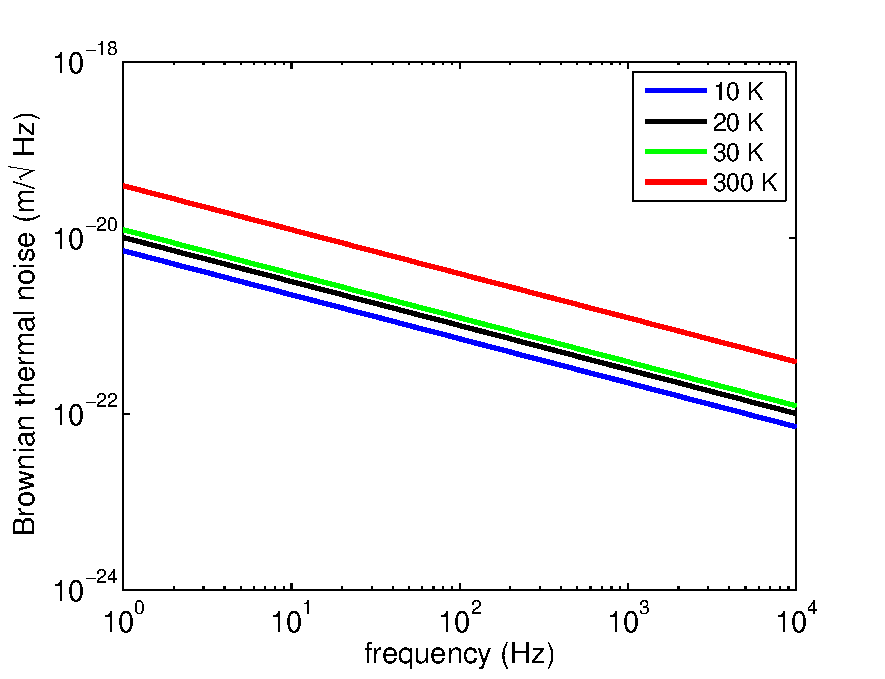
\includegraphics[width=0.49\linewidth]{Sec_Optics/coating_low_TN.pdf}}
\subfigure[]{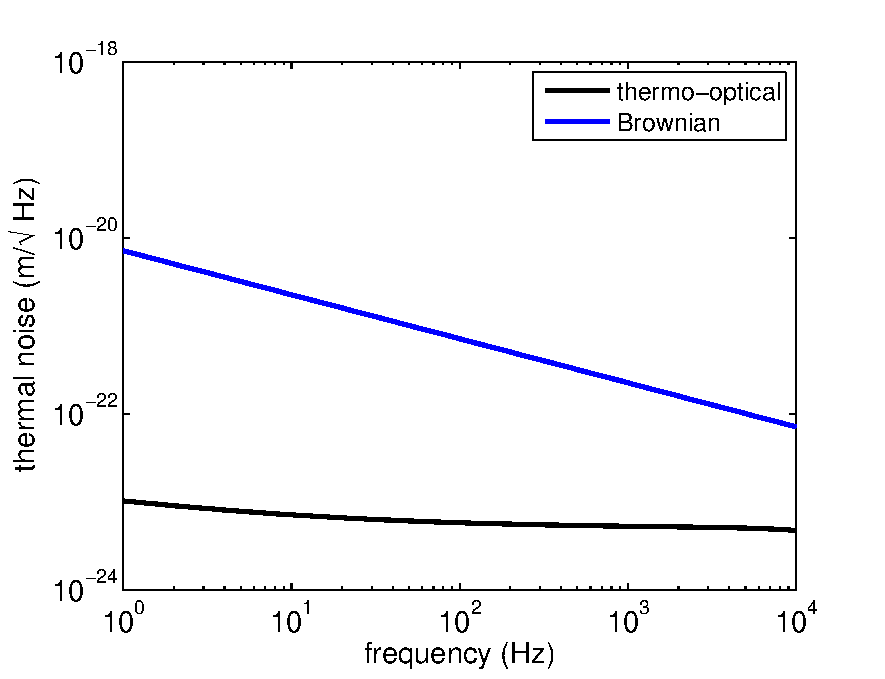
\includegraphics[width=0.49\linewidth]{Sec_Optics/coating_low_TN_TO.pdf}}
\end{center}
\caption{(a)~--~Comparison of coating Brownian noise at different temperatures. (b)~--~Comparison of coating thermo-optical and Brownian noise at room temperature. Both calculations assume a 18 doublet alternating silica-tantala quarter wavelength layer with a $\lambda/2$-endcap. The coating is assumed to be put on a silicon substrate. A wavelength of 1550\,nm was used for the estimates.}
\label{fig:coat_TN}
\end{figure}


Figure~\ref{fig:coat_TN} compares the Brownian and thermo-optical noise levels of different coatings at low temperatures and room temperature. Parameters are used from tables~\ref{tab:summary14}, \ref{tab:tn_T_param}, \ref{tab:tn_param} and \ref{tab:Coat_param}. A direct comparison at 10\,K reveals that the thermo-optical noise is much smaller than the coating Brownian noise. This statement is also true for higher temperatures which makes thermo-optical noise not a dominating source of total thermal noise of a reflective component for a gravitational wave detector.

\longetbox{h}{box:optemp}{Operational Temperature of ET-LF}{The design temperature of the low frequency interferometer of ET was chosen to be 10\,K. This value arises directly from different restrictions. From a thermal noise point of view the lowest possible temperature would be desirable. However, this collides with the necessary heat removal through the suspension as given in section \ref{sec:mat_lss}. At very low temperatures (well below 10\,K) the thermal conductivity of the suspension materials will be very low and it is impossible to remove the deposit heat from the laser beam through the fibres. The maximum tolerable temperature from a point of view of thermal noise is around 24\,K (see Fig.\,\ref{fig:tn_etlf2}). However, as can be seen from Fig.~\ref{fig:coating_loss_cryo} the currently proposed coating material tantala shows a large loss peak around 18\,K when it is annealed to 600 degrees to improve the optical quality. Thus the final decision has been made to go as low as possible in operational temperature to stay below that dissipation peak that would cause an increased level of coating Brownian noise. A summary of the total mirror thermal noise at different temperatures can be found in the appendix \ref{sec:tn_etlf}.}

The level of coating Brownian noise is additionally larger than the total noise level of the bulk material presented in figure~\ref{fig:bulk_T_TN}. Thus, coating Brownian noise is the most important type of thermal noise of a high reflective mirror and great care must be taken in choosing the optimum operational temperature and the appropriate material combination. Avoiding the mechanical loss peak in amorphous dielectric coatings at around 15 to 30\,K (depending on the actual material, see figure~\ref{fig:coating_loss_cryo}) was one of the strongest reasons for the 10\,K target temperature of the cooled mirrors of the ET-LF detector.

Details of the ongoing and future research in the field of mechanical losses of bulk and coating materials as well as other thermal noise issues are given in section~\ref{sec:RD}.


\FloatBarrier
\subsubsection{Thermal noise estimates for transmittive components}
\label{sec:TN_trans}
%\emph{J. Franc}

The total thermal noise of a transmittive component considers the noise contribution described in the previous subsection and additionally the thermo-refractive noise that occurs from statistical fluctuations of the refractive index $n$ due to its temperature dependence $dn/dT$. A temperature fluctuation produces a small change of $n$ which leads to phase changes detected by the interferometer. The thermo-refractive noise has been calculated by equations given by Braginsky~\cite{Braginsky2004} in addition with correction terms developed by Benthem and Levin~\cite{Benthem2009}.

Taking into account the configuration of Einstein Telescope given in figure~\ref{Fig:opt_lay_over} and table~\ref{tab:summary14} results in the following equation for the thermo-refractive noise (power spectral density) in an interferometer with arm cavities of finesse~$F$:

\begin{align}
S_h(f,T)&=\frac{4}{L^2}\left(\frac{\lambda}{8F}\right)^2 \nonumber \\
&\left(kl \beta\right)^{2} \frac{4k_B T^{2} \kappa}{\left(C\rho\right)^{2}l}
\left(1+\frac{\left(kn\right)^{2}w^{2}}{\left(1+\left(2kn\sqrt{\frac{\kappa}{C
\rho\omega}}\right)^{4}\right)}\right) \int_0^{\infty}{\frac{k_i dk_i}{2\pi} \exp \left(\frac{-w^2k_{i}^{2}}{4}\right) \frac{k_{i}^2}{\omega^2+a^4 k^4 }}, 
\label{eq:Tref}
\end{align}

where
\begin{equation}
k=\frac{2 \pi}{\lambda}
\label{eq:k}
\end{equation}

and 

\begin{equation}
{a}^2=\frac{\kappa}{C\rho}.
\end{equation}

$l$ is the thickness of the input mirror, $\beta$ the thermo-optic coefficient of the substrate material, $T$ is the temperature, $k_B$ the Boltzmanns constant, $\kappa$ the thermal conductivity, $C$ the specific heat, $\rho$ the density of the substrate material, $w$ is the beam radius, $L$ the arm length of the interferometer, and $n$ the refractive index of the substrate material. Details of this equation can be found in~\cite{Franc2010}.

At 300\,K the silica substrate provides the lowest thermo-refractive noise (see figure~\ref{fig:Bulk_Tref_300K}). Substrate materials with a low thermo-optic coefficient show a low thermo-refractive noise. As a numerical result, for silica, sapphire and silicon, it is respectively $8\times10^{-6}$, $1.3\times10^{-5}$ and $5.15\times10^{-5}$. 

\begin{figure}[!h]
\begin{center}
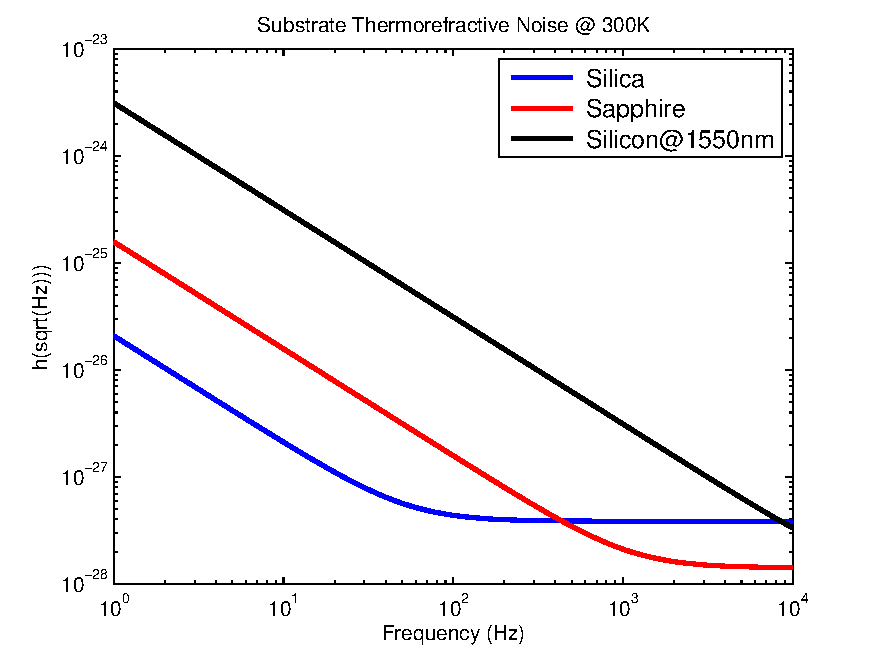
\includegraphics[width=0.49\linewidth]{Sec_Optics/Bulk_Tref_comp_300K.pdf}
\caption{Substrate thermo-refractive noises for silica, sapphire and silicon at room temperature.}
\label{fig:Bulk_Tref_300K}
\end{center}
\end{figure}

Then, the thermo-refractive noise is compared for silicon and sapphire as the most promising test mass materials at cryogenic temperatures. The substrate thermo-refractive noise is largely dependent on the thermo-optic coefficient. This value has been measured for sapphire at low temperatures and reaches $9\times 10^{-8}\,\mathrm{K}^{-1}$ below 4\,K~\cite{Tomaru2002a}. For silicon the parameter is not very well known. The only currently literature source available reports values of $n$ and $dn/dT$ down to 30\,K~\cite{Frey2006}. However, the values reported for $dn/dT$ do not agree with the slope of the $n(T)$ curve of the same reference. Thus, the knowledge of the parameter is strongly limited. At temperatures around 20\,K a value of $1\times10^{-6}\,\mathrm{K}^{-1}$ can be assumed as an upper limit of $dn/dT$ based on the experimental values given in~\cite{Frey2006}. At even lower temperatures it is reasonable to assume a further decrease of the value due to thermodynamical assumptions: at 0\,K all temperature dependent properties have to become constant---thus the temperature derivative has to vanish.

Figure~\ref{fig:Tref_a} shows the thermo-refractive noise of silicon and sapphire at 10\,K based on equation~(\ref{eq:Tref}) given above. The $dn/dT$ for silicon is assumed as $1\times10^{-6}\,\mathrm{K}^{-1}$ and the $dn/dT$ for sapphire is $9\times10^{-8}\,\mathrm{K}^{-1}$.

\begin{figure}[!h]
\begin{center}
\subfigure[]{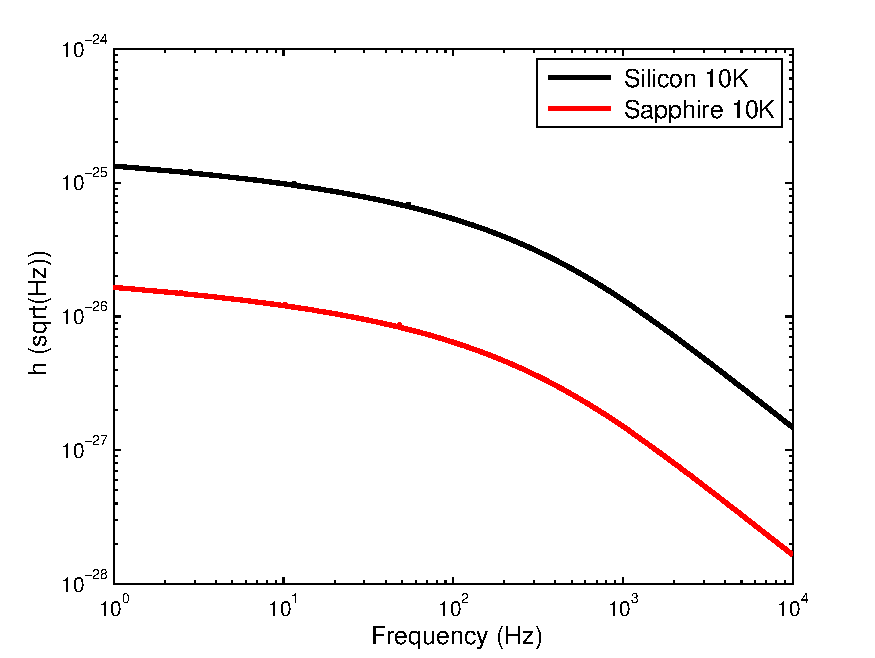
\includegraphics[width=0.49\linewidth]{Sec_Optics/Comp_SiandSa.pdf}\label{fig:Tref_a}}
\subfigure[]{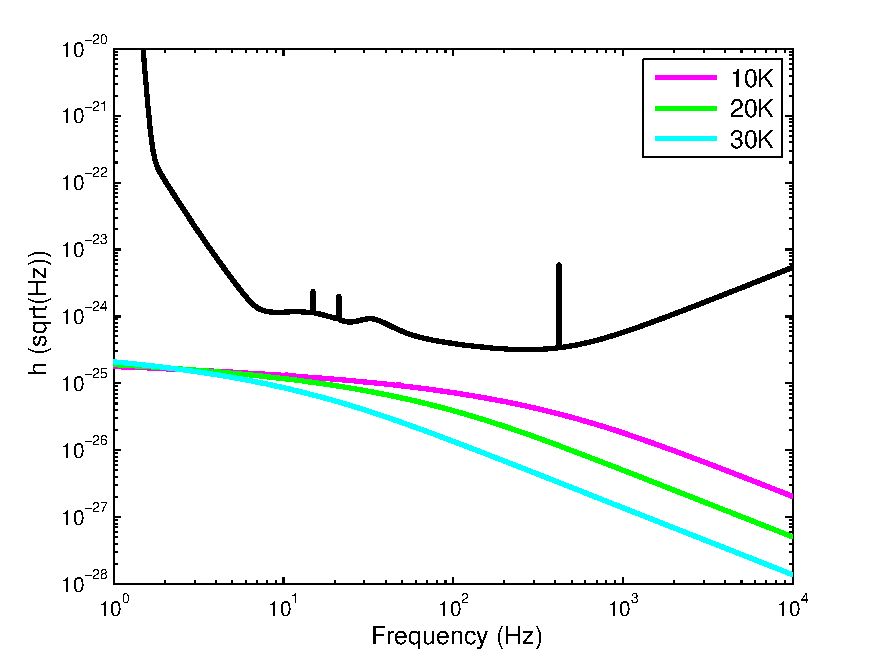
\includegraphics[width=0.49\linewidth]{Sec_Optics/Comp_Temp_TRef.pdf}\label{fig:Tref_b}}
\caption{(a)~--~Substrate thermo-refractive noise of silicon and sapphire at 10\,K (beam size: 9\,cm). (b)~--~Substrate thermo-refractive noise of silicon at 10\,K, 20\,K, 30\,K ($dn/dT$ unchanged:\ $1\times10^{-6}\,\mathrm{K}^{-1}$).}
\end{center}
\end{figure}

Sapphire shows a very small thermo-refractive noise due to its small thermo-refractive coefficient $\beta$. Although it is higher, the thermo-refractive noise of a silicon substrate is also very low and should not affect the total thermal noise of the system. The operational frequency of the LF detector is between 1 and 250\,Hz. Above this frequency the HF detector takes over and limits the sensitivity of the Einstein Telescope. It is expected that experimental values for the thermo-refractive coefficient of silicon is even lower than the one given here (see section~\ref{sec:RD}).

Figure~\ref{fig:Tref_b} shows the evolution of the thermo-refractive noise for different temperatures (10\,K, 20\,K, 30\,K). It shows that the thermo-refractive noise decreases with the temperature. Thus, operating at the highest possible temperature that allows a low thermal noise operation is preferred. This leads to a possible optimization process.

\FloatBarrier
\subsubsection{LF interferometer large mirror definition}
%\emph{Author(s): J. Franc}\\ 
\label{sec:LF_mirror_def}

The Einstein Telescope detector is split into two interferometers (ET-LF and ET-HF) due to thermal noise and heating reasons. The ET-LF detector assumes a beam radius size of 9\,cm, corresponding to an effective test mass diameter of 45-50\,cm, but at the same time keeps the overall test mass weight at about 210\,kg~\cite{Hild2010b} with sufficient thickness.
This mass leads to a thickness for a future silicon test mass of approximately 46-50\,cm. The thickness would drop to about 30\,cm for sapphire due to the higher material density. For the substrate, the thermo-refractive noise is dependent on the thickness of the mirror. 

\begin{figure}[!h]
\begin{center}
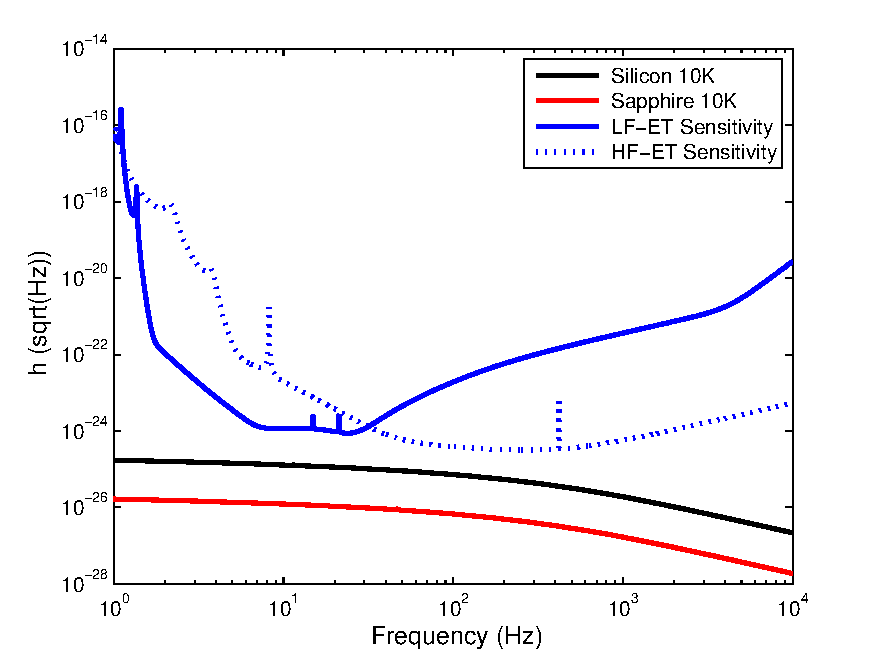
\includegraphics[width=0.49\linewidth]{Sec_Optics/LFSiandSa.pdf}
\caption{Substrate thermo-refractive noise of silicon ($w=9$\,cm, thickness~50\,cm) and sapphire ($w=9$\,cm, thickness~50\,cm) substrate compared to the ET-D sensitivity.}
\label{fig:LFSiandSa}
\end{center}
\end{figure}

Figure~\ref{fig:LFSiandSa} shows that the thermo-refractive noise of silicon and sapphire is well below the ET sensitivity target. Therefore, we can foresee that the assumed dimensions are possible and promising. A plot of all the thermal noises for silicon and sapphire is shown in Figure~\ref{fig:SiandSa}. 

\begin{figure}[!h]
\begin{center}
\subfigure[]{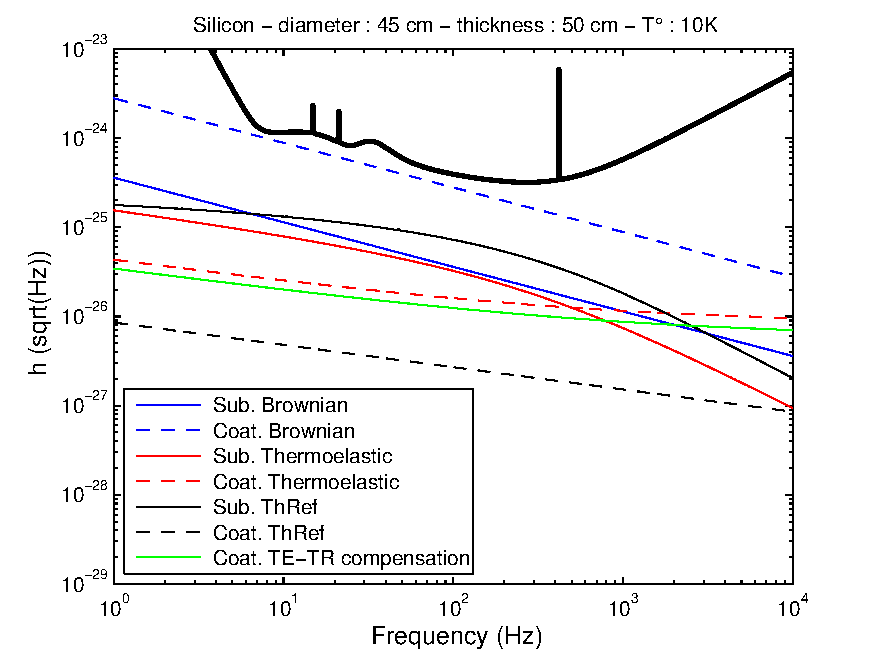
\includegraphics[width=0.49\linewidth]{Sec_Optics/Simirror.pdf}}
\subfigure[]{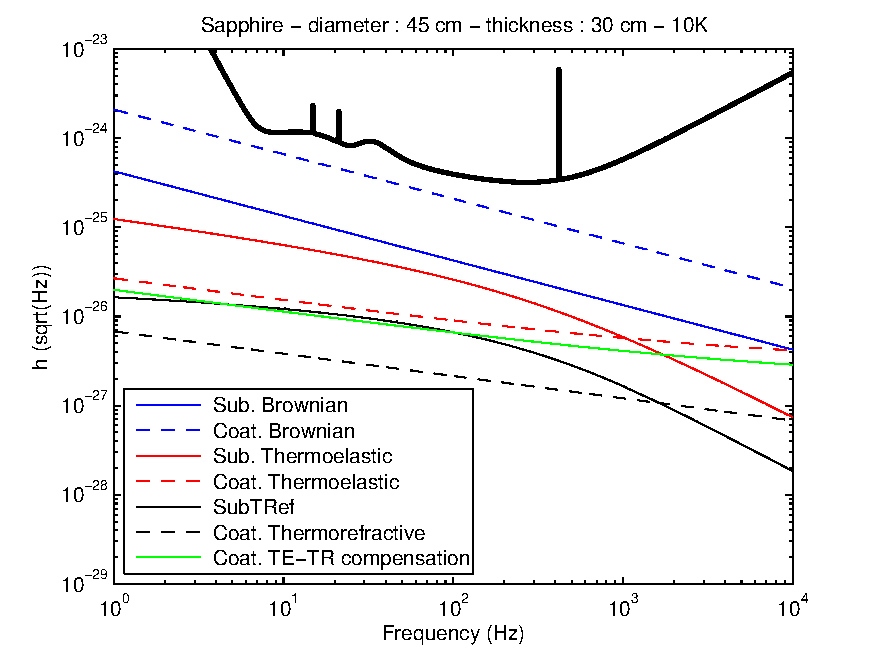
\includegraphics[width=0.49\linewidth]{Sec_Optics/Samirror.pdf}}
\caption{(a)~--~Thermal noise contribution for a silicon mirror ($w=9$\,cm, thickness 50\,cm, $T=10$\,K). (b)~--~Thermal noise contribution for a sapphire mirror ($w=9$\,cm, thickness 30\,cm, $T=10$\,K).}
\label{fig:SiandSa}
\end{center}
\end{figure}

For a silicon mirror, thermal noise is dominated by the coating Brownian noise and the substrate thermo-refractive noise. Coating Brownian noise is, in reality, higher than all other noises considered but still below the ET-LF sensitivity target. For a sapphire substrate, coating Brownian noise is also the highest thermal noise. Therefore, a cooled silicon (or sapphire) mirror provides a low enough thermo-refractive noise in the frequency band covered by the LF detector. 

In conclusion, both materials---sapphire and silicon---provide low thermo-refractive noise levels that are compatible with the requirements for the Einstein Telescope. An exact estimate of the thermo-refractive noise level of silicon will not be possible until the thermo-refractive coefficient is measured for different types of silicon. It can be expected that this parameter strongly depends on the level of doping. Several institutions are currently working on experiments to extend the existing parameters to temperatures below 30\,K.


%\emph{Author(s): R. Nawrodt} \\

Based on the calculations presented in sections~\ref{sec:TN_refl} and \ref{sec:TN_trans} it is now possible to give an overall estimate of the expected thermal noise from the optical components of the ET-LF detector. The total estimate is based on the simplified sketch of the ET-LF detector in figure~\ref{Fig:opt_lay_over}. The input coupler of the cavity as well as the end test mass are cooled to cryogenic temperatures around 10\,K. The beam splitter is operated at room temperature. 

In order to achieve a good thermal noise performance of the optical components a large beam radius $w$ as large as 90\,mm is needed. This requires the use of large diameter bulk samples to avoid large clipping losses. This requirement lead to a typical substrate diameter of 50\,cm. In addition the suppression of radiation pressure noise requires large masses---for the ET-D design a mass of 211\,kg is needed. In combination with the maximum available diameter of a potential silicon test mass material this leads to a required minimum thickness of 46\,cm for the optical components involved in the arm cavities (end test mass and input coupler). A further increase of the thickness will reduce radiation pressure noise further---however, it will increase the thermo-refractive noise of the input test mass. 

The option to use sapphire as a test mass material seems to be strongly limited by the availability of the materials. So far, it is not expected that by the time ET will be built sapphire test masses with a required diameter of 50\,cm will be available on the market. Thus, all estimates in this section are based on the choice of silicon as a test mass material---although sapphire will totally satisfy all noise demands if operated at the same temperature and if it is available in the same geometry.

Figure~\ref{fig:ET_LF_ETM_total} shows the total thermal noise of an end test mass cavity mirror for ET. The calculations are based on the properties presented in tables~\ref{tab:summary14}, \ref{tab:tn_T_param}, \ref{tab:tn_param}, and \ref{tab:Coat_param}. A silicon test mass with a diameter of 50\,cm and a thickness of 46\,cm was assumed to be operated at 10\,K. The ETM uses 18 $\mathrm{\lambda/4}$-doublets of tantala/silica layers and the ITM 9 $\mathrm{\lambda/4}$-doublets of tantala/silica to form the cavity. While the laser beam reads out the surfaces of the cavity mirrors 

\begin{equation}
N=2/\pi F
\label{eq:red_factor}
\end{equation}

times ($F$~--~finesse of the cavity) it only senses the thermo-refractive noise of the ITM twice (input and output of the cavity). This reduction factor is included for the ITM and the thermo-refractive noise recalculated as an effective displacement noise for comparison.

\begin{figure}[!h]
\begin{center}
\subfigure[\label{fig:ET_LF_ETM_total}]{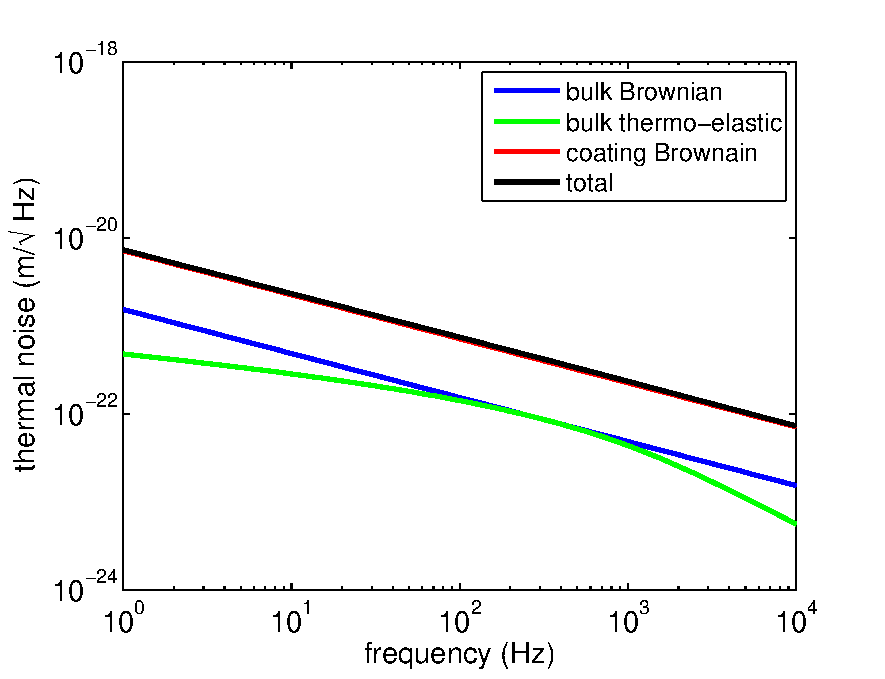
\includegraphics[width=0.49\linewidth]{Sec_Optics/ET_LF_ETM_TN.pdf}}
\subfigure[\label{fig:ET_LF_ITM_total}]{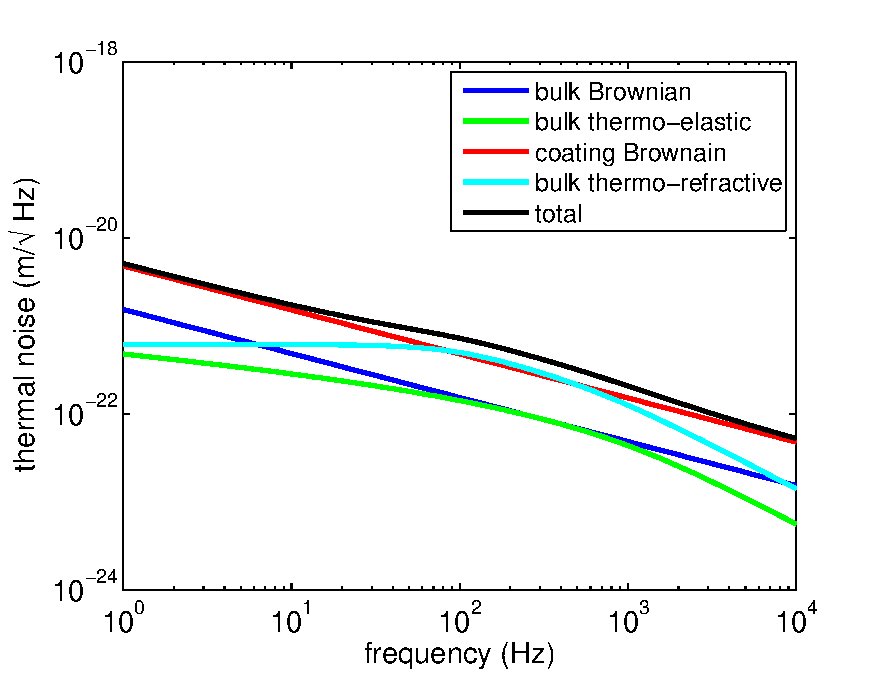
\includegraphics[width=0.49\linewidth]{Sec_Optics/ET_LF_ITM_TN.pdf}}
\end{center}
\caption{Total thermal noise of an end test mass~(a) and an input test mass~(b) of the arm cavity of ET-LF. Both substrates are assumed to be made of silicon with a diameter of 50\,cm and a thickness of 46\,cm. The operational temperature is 10\,K. The ETM is equipped with 18 $\mathrm{\lambda/4}$-doublets of a tantala/silica high-reflective stack while the ITM is coated with 9 $\mathrm{\lambda/4}$-doublets to achieve a transmission of about 7000\,ppm.}
\end{figure}

For both---the ETM and the ITM---the coating Brownian noise dominates over all frequencies. For the input test mass the required 46\,cm thickness leads already to significant contributions from the thermo-refractive noise. The uncorrelated sum of the different noise contributions in the ETM and the ITM can be used as a good estimate for the total thermal noise contribution of one arm cavity. 

An additional noise source in the interferometer is the beam-splitter. Due to the fact that this element is situated outside the arm cavities its thermal noise contribution to the overall thermal noise of the detector is again reduced by the factor given in eq.~(\ref{eq:red_factor}). Thus, cooling might not be needed for this component. The beam splitter is assumed to be made of fused silica and operated at room temperature. The different thermal noise contributions based on the equations given in the previous sections are summarised in figure~\ref{fig:ET_LF_BS_TN}. The beam splitter is assumed to be coated with 3 $\mathrm{\lambda/4}$-doublets of tantala/silica as an upper limit calculation. The thickness of the beam splitter is 10\,cm and the aspect ratio is kept similar to the end test masses. 

\begin{figure}[!h]
\begin{center}
\subfigure[\label{fig:ET_LF_BS_TN}]{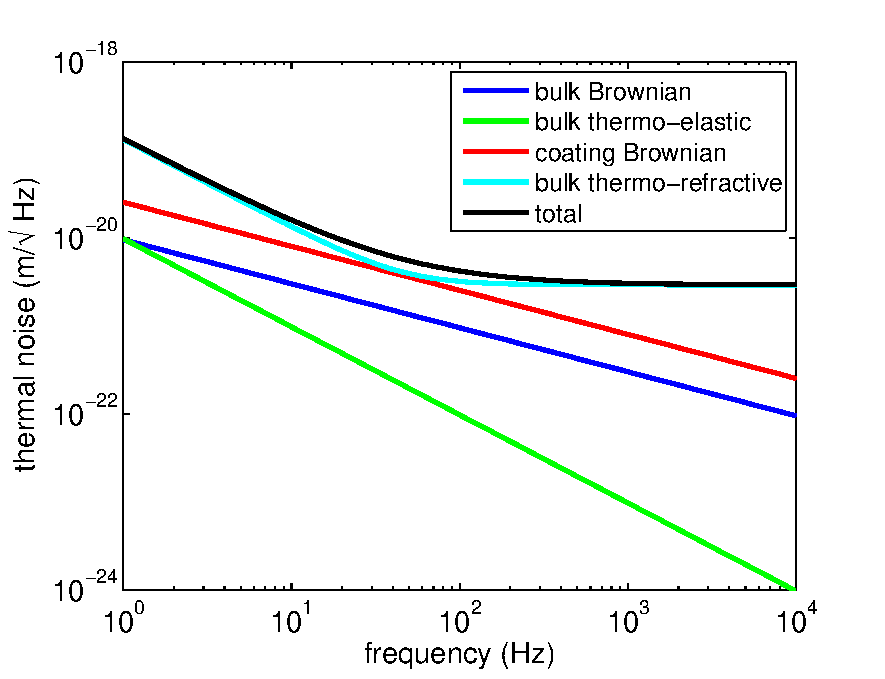
\includegraphics[width=0.49\linewidth]{Sec_Optics/ET_LF_BS_TN.pdf}}
\subfigure[\label{fig:ET_LF_BS_total}]{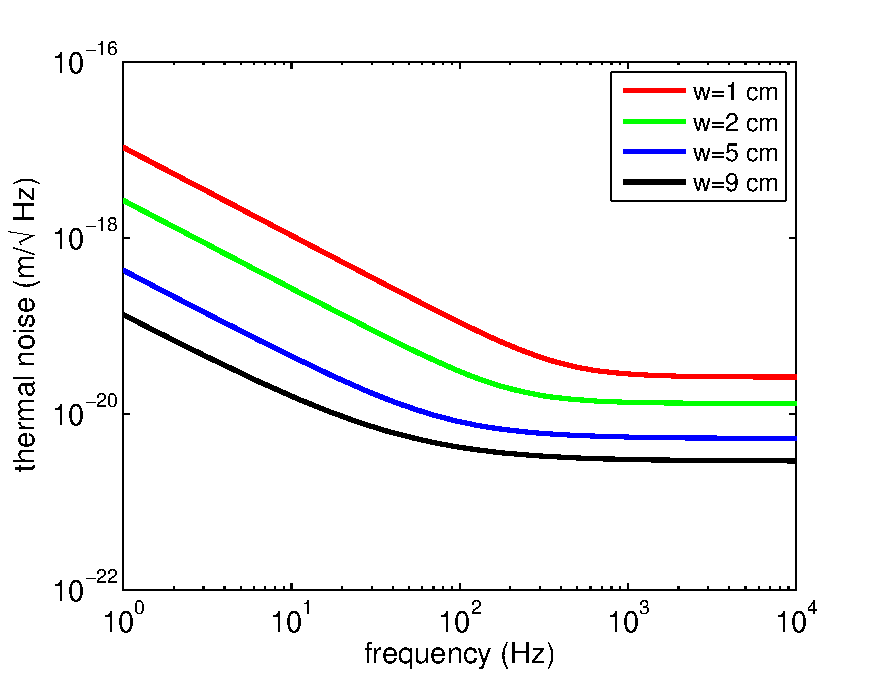
\includegraphics[width=0.49\linewidth]{Sec_Optics/ET_LF_BS_total.pdf}}
\end{center}
\caption{(a)~--~Summary of the different thermal noise sources in a potential ET-LF beam splitter made of fused silica and operated at room temperature. (b)~--~Evolution of the total thermal noise of the beam splitter with different beam radii at the beam splitter.}
\end{figure}

The thermo-refractive contribution from the beam-splitter is based on the calculation by Benthem and Levin for GEO600~\cite{Benthem2009}. Thermo-refractive noise is the most dominating noise source of the beam splitter due to the very low mechanical loss of fused silica at room temperature and the small number of coating layers. If the beam radius of the laser beam at the beam splitter is further reduced, thermo-refractive noise increases as shown in fig.~\ref{fig:ET_LF_BS_total}. This reduction of the beam radius might be beneficial to reduce the necessary size of the beam splitter. Due to the fact that the beam splitter is operated under an angle the necessary size is increased compared to an end mirror. These mirrors are currently already designed to be at or close to the edge of what is and will be available by the time ET will be built. Thus, a reduction of the dimensions of the beam splitter is needed. 
 
Combining all noise contributions from the two arm cavities and the beam splitter (incoherent sum) leads to an estimate of the total thermal noise contribution for ET-LF, which is given in figure~\ref{fig:ET_LF_total_TN} for different beam radii at the beam splitter.

\begin{figure}[!h]
\begin{center}
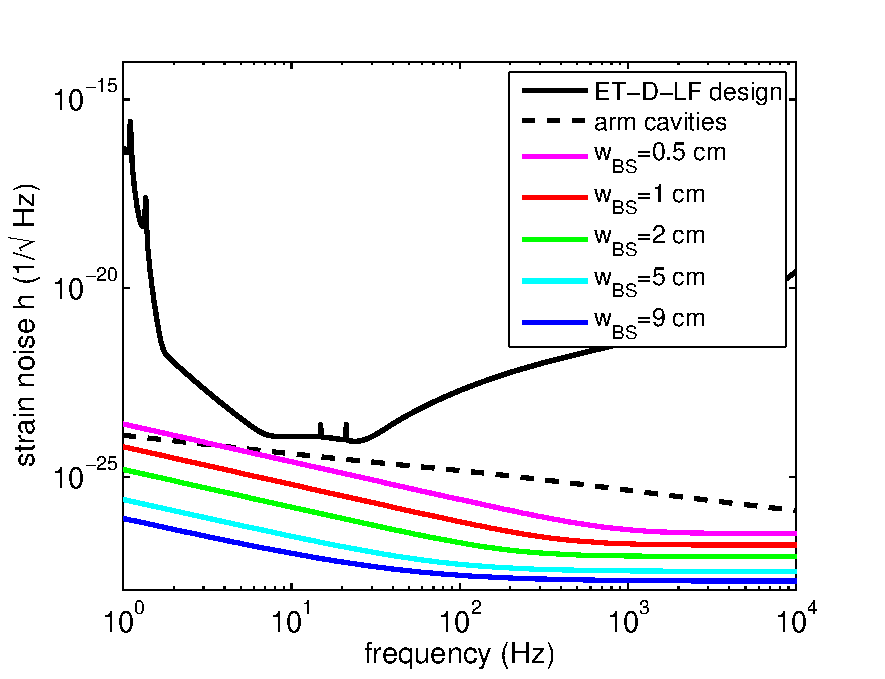
\includegraphics[scale=0.7]{Sec_Optics/ET_LF_noise.pdf}
\end{center}
\caption{Total thermal noise arising from the optical components of ET-LF for different beam radii at the beam splitter.}
\label{fig:ET_LF_total_TN}
\end{figure}

It is obvious that the main thermal noise contribution comes from the arm cavities. Even if the beam radius at the beam splitter is chosen to be as small as 0.5\,cm the noise contribution from the beam splitter is smaller than the contribution from the arm cavities. This relaxes the demands for the size of the beam splitter and the thermal noise contribution of the beam splitter is in agreement with the proposed beam diameter at the beam splitter of 6\,mm.

\FloatBarrier
\subsubsection{HF interferometer large mirror definition}
%\emph{Author(s): J. Franc \\}

Fused silica is the material of choice for the high frequency detector operating at room temperature. Fused silica is one of the most commonly used materials in optics and has been improved during many decades. Appropriate polishing methods exist to obtain a very high surface quality. Fused silica has remarkable properties at room temperature: low mechanical loss (see section~\ref{app:mechdat}) which leads to a small substrate Brownian noise, and an exceptional low coefficient of thermal expansion (see section~\ref{app:thermdat}) which results in a small thermo-elastic noise.

\begin{table}[!h]
\begin{center}
\begin{tabular}{|c|c|} \hline
Parameter & ET-HF \\ \hline
temperature & 290\,K \\
arm length & 10\,km \\ 
mirror material & Fused silica \\
mirror diameter & 62\,cm \\
mirror thickness & 30\,cm \\
mirror mass & 200\,kg \\
laser wavelength & 1064\,nm \\
beam shape & TEM$_{00}$ \\
beam radius & 12\,cm \\
coating high index & $\mathrm{Ti:Ta_2O_5}$ \\
coating low index & $\mathrm{SiO_2}$ \\ 
\hline
\end{tabular}
\end{center}
\caption{Summary of the parameters used for the thermal noise estimate of the HF interferometer.}
\label{tab:HF_dat}
\end{table}

The assumed parameters for the ET-HF interferometer are listed in Table~\ref{tab:HF_dat}. The mirror geometry was chosen so that the mass reaches 200\,kg to suppress radiation pressure noise and that the mirror geometry causes only 1\,ppm diffraction loss at its boundaries~\cite{Vinet2007}. For the sake of simplicity, in this estimates a TEM$_{00}$ beam has been taken into account, considering the use of LG$_{33}$ as an option for the HF interferometer. Using LG$_{33}$ modes will further reduce thermal noise. However, it will be shown that the currently assumed geometry is already compliant with the ET-HF sensitivity curve if a TEM$_{00}$ mode is assumed.

In order to compare the behaviour of different substrate materials the thermal noise of a high reflectivity mirror was calculated using the same `standard' coating and different substrate materials. The `standard' coating is a multilayer $\mathrm{(HL)_{17}HLL}$ coating made of $\mathrm{Ti:Ta_2O_5}$ and $\mathrm{SiO_2}$ quarter wavelength layers. On a fused silica substrate this coating corresponds to a transmission of 6\,ppm. The lowest mechanical loss experimentally observed has been considered for the coating materials (see section~\ref{app:mechdat}). The result of this comparison is shown in Figure~\ref{fig:substrate_comp}. The graph plots different noise sources in the substrate materials as well as their coatings. 

\begin{figure}[!h]
\begin{center}
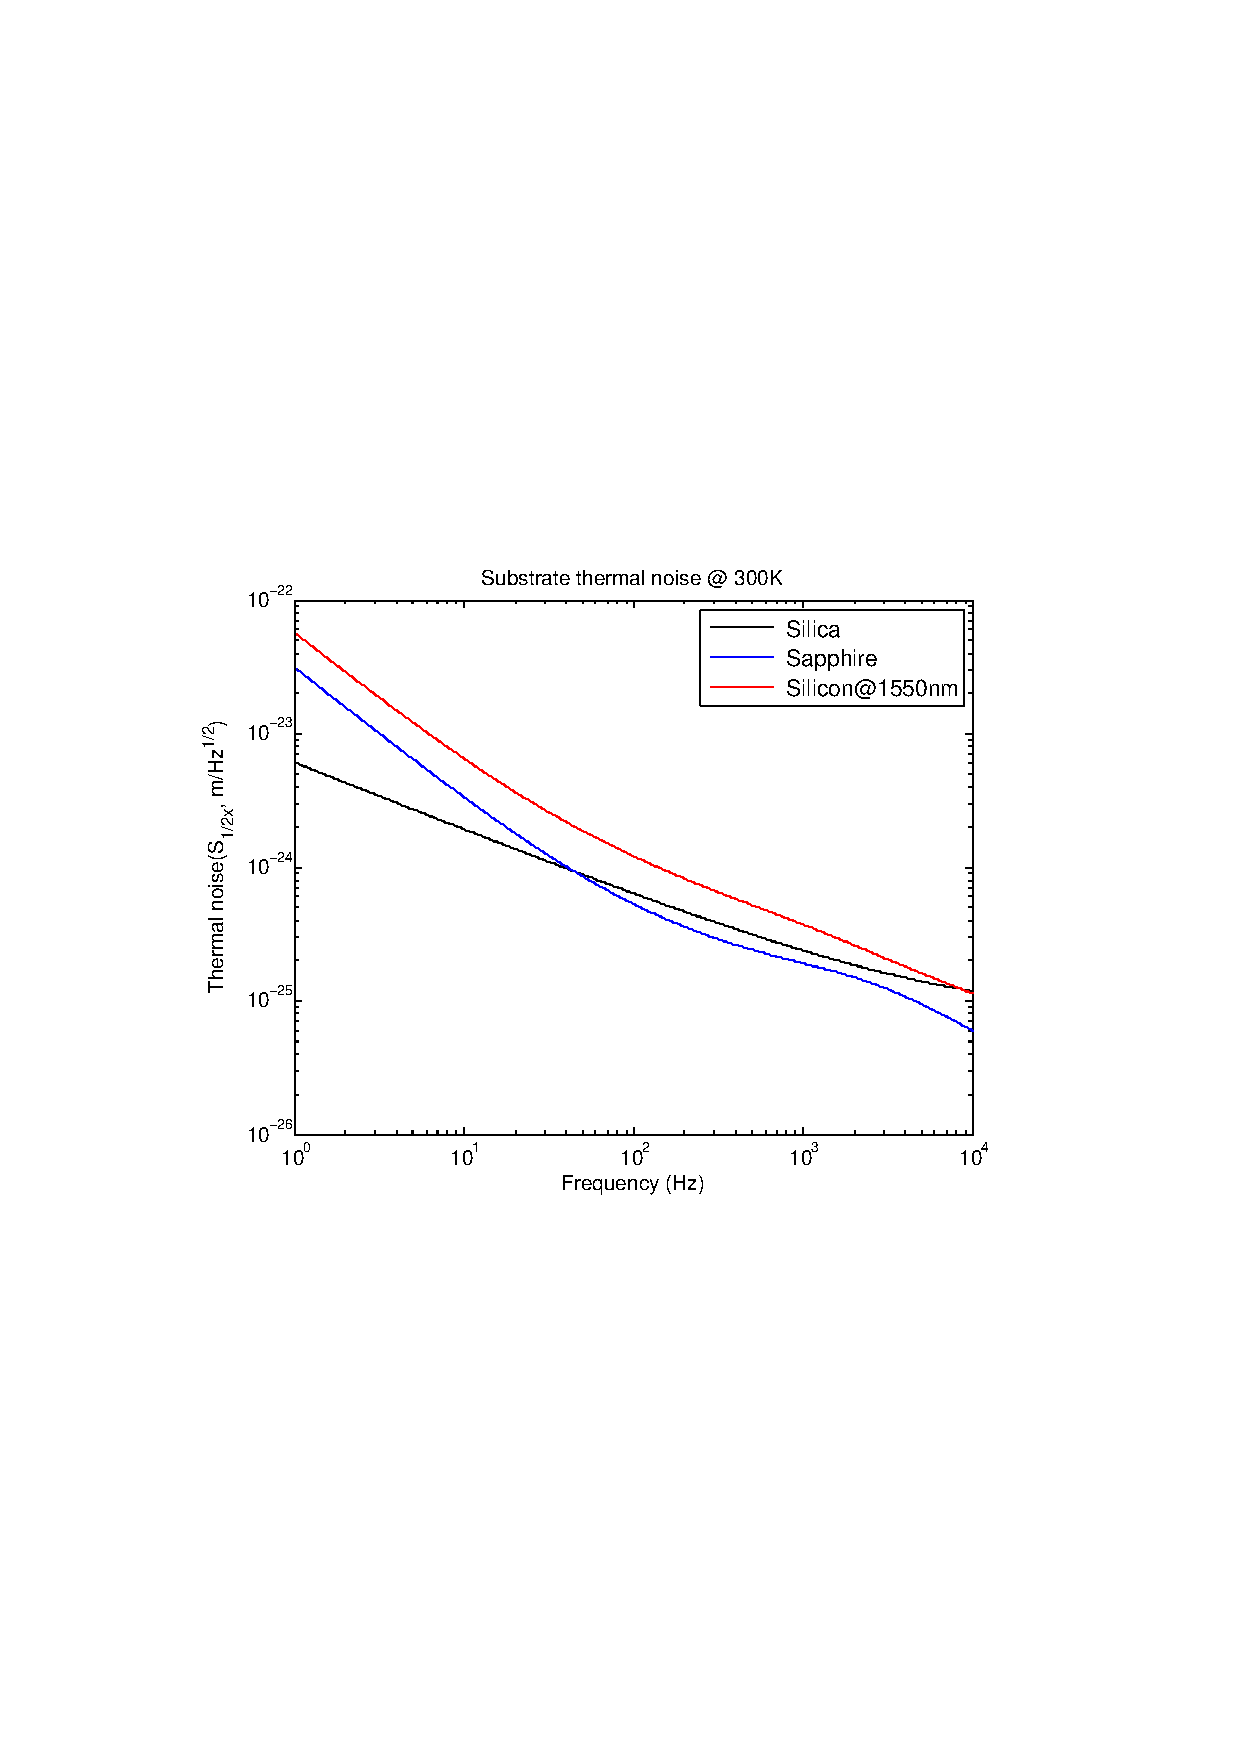
\includegraphics[width=0.49\linewidth]{Sec_Optics/substrate_comp.pdf}
\caption{Total thermal noise of three different substrates at 300\,K: silica, sapphire, and silicon at 1550\,nm. }
\label{fig:substrate_comp}
\end{center}
\end{figure}

At 300\,K, the total thermal noise for silicon is limited by two substrate thermal noises: substrate Brownian noise at high frequencies and substrate thermo-elastic noise at low frequencies. Sapphire must also be discarded due to its large thermo-elastic noise at low frequencies. Therefore, the most adapted substrate at room temperature is fused silica. In this case, coating limits the sensitivity of the future detectors only through its Brownian thermal noise. 

\paragraph{Mirror coating}
%\emph{Author(s): J. Franc} \\ 

As explained above, the total thermal noise of the test masses is a combination of coating Brownian, substrate Brownian, substrate thermo-elastic, substrate thermo-refractive, and thermo-optic noise. Taking into account these five noise sources, the coating Brownian noise is the most important one and can limit the sensitivity target. A state-of-the-art of different coating material have been realized in order to compare different combination of multilayer stacks.  

Figure~\ref{fig:coating} shows the total thermal noise for different coatings on a silica substrate at room temperature. The calculations are based on the currently best available data of the materials (table~\ref{tab:Coat_param}). Each coating corresponds to a transmission of 6\,ppm on a fused silica mirror. Therefore, all multilayers are different according to materials taken into account.

We need:

\begin{itemize}
	\item $\mathrm{(HL)_{17}HLL}$ for a coating made of $\mathrm{Ti:Ta_2O_5}$ and $\mathrm{SiO_2}$ quarter wavelength layers,
	\item $\mathrm{(HL)_{13}HLL}$ for a coating made of $\mathrm{TiO_2}$ and $\mathrm{SiO_2}$,
	\item $\mathrm{(HL)_{13}HLL}$ for a coating made of $\mathrm{Nb_2O_5}$ and $\mathrm{SiO_2}$,
	\item $\mathrm{(HL)_{16}HLL}$ for a coating made of $\mathrm{ZrO_2}$ and $\mathrm{SiO_2}$,
	\item $\mathrm{(HL)_{24}HLL}$ for a coating made of $\mathrm{Ti:Ta_2O_5}$ and $\mathrm{Al_2O_3}$, and
	\item $\mathrm{(HL)_{22}HLL}$ for a coating made of $\mathrm{ZrO_2}$ and $\mathrm{Al_2O_3}$.
\end{itemize}

According to the refractive index of the material the number of layers can vary by a factor of two. 

\begin{figure}[!h]
\begin{center}
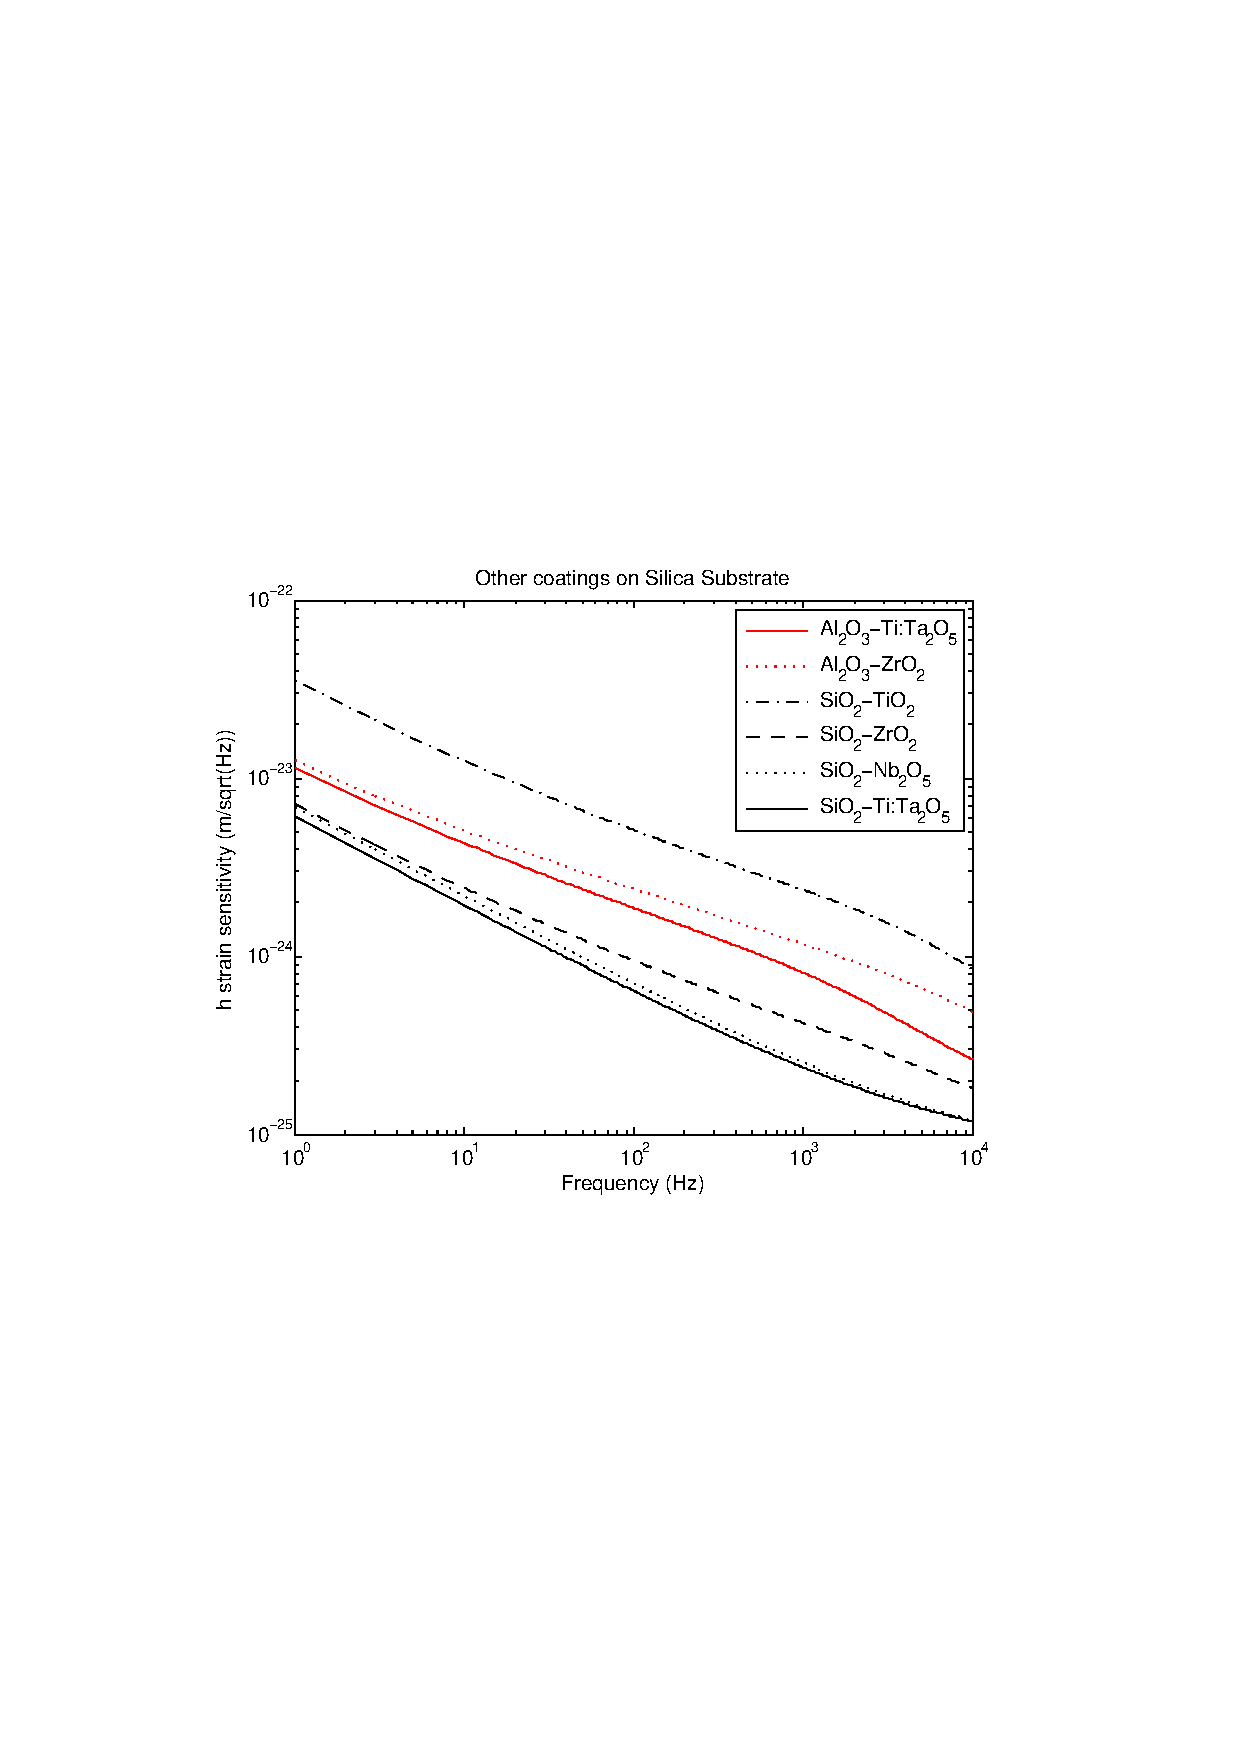
\includegraphics[bb=100 270 500 570,width=0.49\linewidth]{Sec_Optics/coating.pdf}
\end{center}
\caption{Comparison of the thermal noise of different coating materials on a fused silica substrate at room temperature.}
\label{fig:coating}
\end{figure}

There is a clear advantage for the $\mathrm{SiO_2-Ti:Ta_2O_5}$ coating showing the lowest coating thermal noise.
The results obtained for $\mathrm{SiO_2-Nb_2O_5}$ and $\mathrm{SiO_2-ZrO_2}$ are encouraging as well. However, if we include the optical absorption of the coatings, the use of the standard coating is even more strongly supported. So far, there is no better coating to be used at room temperature than the $\mathrm{Ti:Ta_2O_5-SiO_2}$. 

\begin{figure} [!h]
\begin{center}
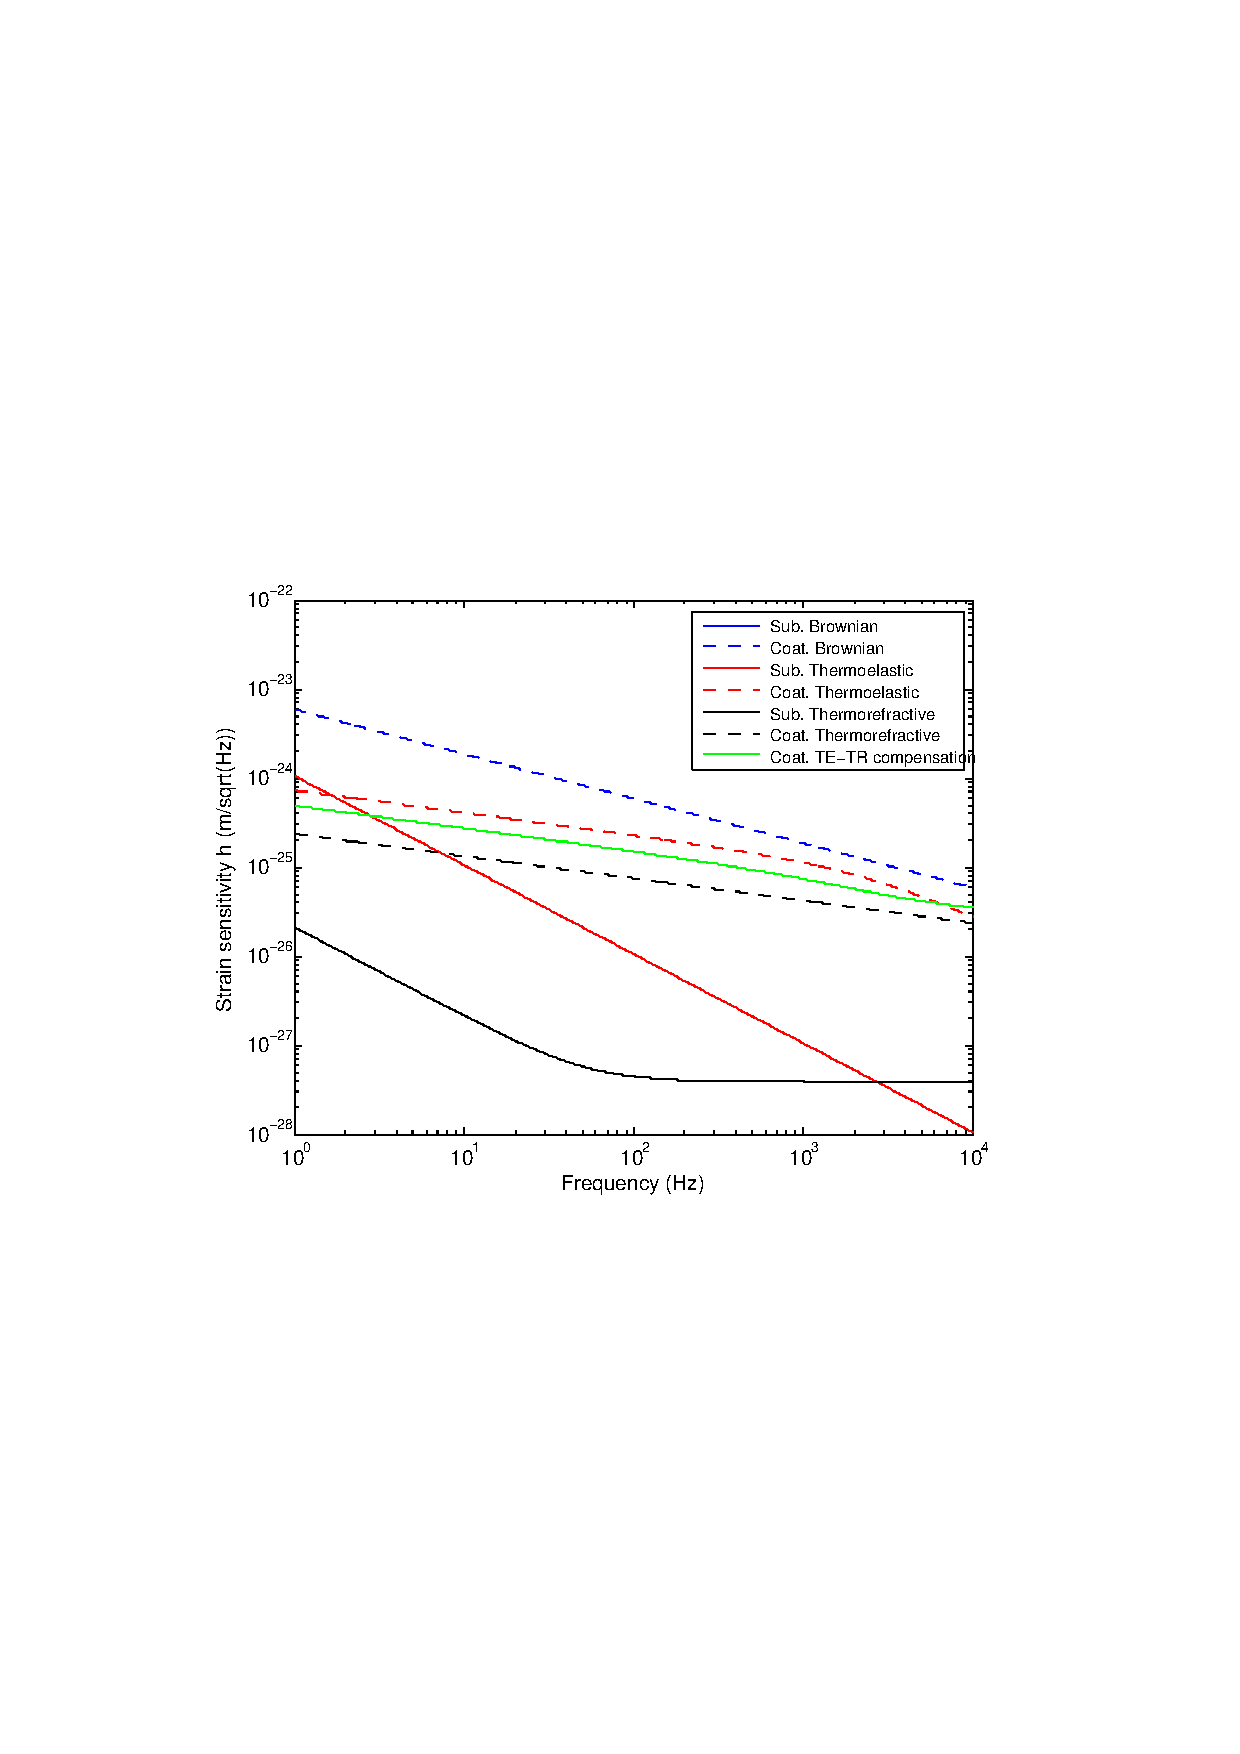
\includegraphics[bb=100 270 500 570,width=0.49\linewidth]{Sec_Optics/silicaTTN.pdf}
\end{center}
\caption{Contribution of the different thermal noises for a fused silica mirror at room temperature.}
\label{fig:silicaTTN}
\end{figure}

In conclusion, we have evaluated the total mirror thermal noise at room temperatures by implementing a model that includes Brownian, thermo-elastic and thermo-refractive noise. From the different calculations we have presented based on the parameters listed above we draw the conclusion that fused silica is the best test mass material for the high frequency detector of the 3rd generation GWD. The optimized mirror for the HF interferometer is, at present, a fused silica test mass with a diameter of 62\,cm and a thickness of 30\,cm.

%------
%\FloatBarrier
\subsubsection{Mirror surface defects}
\label{sec:msurface}

%\emph{Author(s): M. Galimberti, K. Kokeyama}\\ 

Here we discuss investigations of mirror surface defects in order to understand their effects on cavity resonance and losses, and to define requirements for surface polishing. For convenience, the mirror surface deviations from the perfect surface can be classified into two categories, depending on their spatial frequencies. Defects in the high frequency range (above a few hundred m$^{-1}$) will scatter light outside the cavity and thus generate cavity losses and scattering noise. Defects in the spatial low frequency range (between 1 and 100\,m$^{-1}$) may induce resonance of unwanted modes in the cavity, and thus degrade the mode purity inside the cavity.
 
 % from LMA presentations in Jena, Kyoto, and Budapest (2010)
The ET arm cavities were simulated by FFT propagation using the simulation software \emph{SIESTA}~\cite{Caron1999}. Artificial mirror maps were applied to both mirrors of the cavity. The artificial maps were randomly generated in order to reproduce a defect distribution similar to that found in actual VIRGO and LIGO mirrors~\cite{Galimberti2010a, Galimberti2010, Galimberti2010b}.  

Table~\ref{tab:msurface} shows the cavity gain and round-trip losses for the fundamental mode resonating in the cavity (wavelength of 1064 or 1550\,nm), with varying RMS flatness of the surface defects. The distribution of defects considered here goes as $f^{-2}$, where $f$ is the spatial frequency. It has been shown in~\cite{Galimberti2010b} that such a distribution, with a RMS of 1.0\,nm, overestimates the low-frequency defects with respect to what has already been obtained for the Advanced LIGO mirrors. Therefore the surfaces obtained by current polishing techniques seem already good enough to obtain reasonably small round-trip losses for the fundamental mode. Using a wavelength of 1550~nm is particularly favourable from this point of view (smaller losses).
 
\begin{table}[h]
\begin{center}
\begin{tabular}{ccccc}
%
\hline
RMS flatness 	& \multicolumn{2}{c}{TEM$_{00}$ 1064\,nm} 	& \multicolumn{2}{c}{TEM$_{00}$ 1550\,nm}\\
				& cavity gain 	& r.t.\ losses [ppm]			& cavity gain 	& r.t.\ losses [ppm]		\\
\hline
0\,nm 			& 567.4			& 2							& 567.4			& 3						\\
0.5\,nm			& $564.5\pm0.9$	& $20\pm6$					& $566.7\pm0.3$	& $7\pm2$				\\
1.0\,nm			& $555.9\pm3.7$	& $73\pm24$					& $564.4\pm0.9$	& $21\pm6$				\\
\hline
%
\end{tabular}
\end{center}
\caption[Round-trip losses as a function of surface defects]{Cavity gain and round-trip losses for the arm cavities, computed from FFT simulations, as a function of surface defects RMS. The fundamental TEM$_{00}$ mode is considered, for the wavelengths 1064 and 1550\,nm. Data are expressed as mean${}\pm{}$standard deviation on an ensemble of 10 different cavities. For each cavity, random surface maps with a given RMS amount of defects are applied to both mirrors. The random surface maps are generated from a $f^{-2}$ spectral distribution.}
\label{tab:msurface}
\end{table}


The situation for LG$_{33}$ is more delicate. It has been shown~\cite{Galimberti2010b} that LG$_{33}$ is significantly more sensitive than the fundamental mode to surface defects in the low spatial frequency range. Essentially, since a cavity tuned for LG$_{33}$ is degenerate for all modes of order~9, the low-frequency defects may induce the coupling between the injected LG$_{33}$ and the other modes of the same order. Polishing techniques such as corrective coating or ion beam polishing are able to reduce the amount of defects in the low-frequency region, approximately below 100\,m$^{-1}$ (1\,cm$^{-1}$). Ion beam polishing has currently been used for Advanced LIGO, whereas corrective coating is under evaluation for Advanced VIRGO~\cite{Billingsley2011, Bonnand2011}. Preliminary results indicate that a further improvement is required for LG$_{33}$ with respect to the state of the art of such techniques~\cite{Galimberti2010b}. More work is planned to verify the agreement of FFT simulations with experiments on LG$_{33}$ (see section~\ref{sec:thermalnoiseLG}).

% activities in Birmingham.
In addition to the above work, the coupling between higher-order modes
due to mirror surface defects was investigated using a frequency
domain simulation tool, \emph{Finesse}~\cite{bond10}.
In this work, similarly to the simulation mentioned above,
a Fabry-Perot cavity with imperfect mirrors was simulated.
Real surface maps of VIRGO mirrors
were reconstructed by fitting with Zernike polynomials,
and an artificial map was built by a sum of Zernike polynomials.
A LG$_{33}$ beam was injected into a cavity where a surface map
was applied on one of the two cavity mirrors.
The light field inside the cavity was analyzed and found
not only the couplings between the same order,
but also the frequency split of the resonant frequency
which will result in quasi-degenerate modes.

% Next step
The next step is to expand the optical configuration to a realistic topology such as a RSE interferometer in order to obtain practical requirements for the mirror surface. Also, the effects of advanced polishing techniques such as corrective coating or ion beam polishing
need to be better understood.



%% spare parts to be included
%To evaluate competences of each material, the figure \ref{fig:substrates} shows the substrate thermal noise at 10K and 300K for the three different substrates : silica, silicon and sapphire. The thermal noises taken into account for the simulation are the substrate brownian noise and the substrate thermo-elastic noise. we not deal with substrate thermo-refractive noise which will be developed subsequently. The beam size is 8.65 cm. Considering these two noises only, at 300K, the silica is decidedly better than silicon and sapphire substrate. On the other hand, at 10K, silicon and sapphire becomes very good candidate whereas silica is unsuitable.
